% Options for packages loaded elsewhere
% Options for packages loaded elsewhere
\PassOptionsToPackage{unicode}{hyperref}
\PassOptionsToPackage{hyphens}{url}
\PassOptionsToPackage{dvipsnames,svgnames,x11names}{xcolor}
%
\documentclass[
  12pt,
  number,
  doubleblind]{elsarticle}
\usepackage{xcolor}
\usepackage[inner=1in,outer=1in,top=1in,bottom=1in]{geometry}
\usepackage{amsmath,amssymb}
\setcounter{secnumdepth}{5}
\usepackage{iftex}
\ifPDFTeX
  \usepackage[T1]{fontenc}
  \usepackage[utf8]{inputenc}
  \usepackage{textcomp} % provide euro and other symbols
\else % if luatex or xetex
  \usepackage{unicode-math} % this also loads fontspec
  \defaultfontfeatures{Scale=MatchLowercase}
  \defaultfontfeatures[\rmfamily]{Ligatures=TeX,Scale=1}
\fi
\usepackage{lmodern}
\ifPDFTeX\else
  % xetex/luatex font selection
  \setmainfont[]{Times New Roman}
\fi
% Use upquote if available, for straight quotes in verbatim environments
\IfFileExists{upquote.sty}{\usepackage{upquote}}{}
\IfFileExists{microtype.sty}{% use microtype if available
  \usepackage[]{microtype}
  \UseMicrotypeSet[protrusion]{basicmath} % disable protrusion for tt fonts
}{}
\usepackage{setspace}
\makeatletter
\@ifundefined{KOMAClassName}{% if non-KOMA class
  \IfFileExists{parskip.sty}{%
    \usepackage{parskip}
  }{% else
    \setlength{\parindent}{0pt}
    \setlength{\parskip}{6pt plus 2pt minus 1pt}}
}{% if KOMA class
  \KOMAoptions{parskip=half}}
\makeatother
% Make \paragraph and \subparagraph free-standing
\makeatletter
\ifx\paragraph\undefined\else
  \let\oldparagraph\paragraph
  \renewcommand{\paragraph}{
    \@ifstar
      \xxxParagraphStar
      \xxxParagraphNoStar
  }
  \newcommand{\xxxParagraphStar}[1]{\oldparagraph*{#1}\mbox{}}
  \newcommand{\xxxParagraphNoStar}[1]{\oldparagraph{#1}\mbox{}}
\fi
\ifx\subparagraph\undefined\else
  \let\oldsubparagraph\subparagraph
  \renewcommand{\subparagraph}{
    \@ifstar
      \xxxSubParagraphStar
      \xxxSubParagraphNoStar
  }
  \newcommand{\xxxSubParagraphStar}[1]{\oldsubparagraph*{#1}\mbox{}}
  \newcommand{\xxxSubParagraphNoStar}[1]{\oldsubparagraph{#1}\mbox{}}
\fi
\makeatother


\usepackage{longtable,booktabs,array}
\usepackage{calc} % for calculating minipage widths
% Correct order of tables after \paragraph or \subparagraph
\usepackage{etoolbox}
\makeatletter
\patchcmd\longtable{\par}{\if@noskipsec\mbox{}\fi\par}{}{}
\makeatother
% Allow footnotes in longtable head/foot
\IfFileExists{footnotehyper.sty}{\usepackage{footnotehyper}}{\usepackage{footnote}}
\makesavenoteenv{longtable}
\usepackage{graphicx}
\makeatletter
\newsavebox\pandoc@box
\newcommand*\pandocbounded[1]{% scales image to fit in text height/width
  \sbox\pandoc@box{#1}%
  \Gscale@div\@tempa{\textheight}{\dimexpr\ht\pandoc@box+\dp\pandoc@box\relax}%
  \Gscale@div\@tempb{\linewidth}{\wd\pandoc@box}%
  \ifdim\@tempb\p@<\@tempa\p@\let\@tempa\@tempb\fi% select the smaller of both
  \ifdim\@tempa\p@<\p@\scalebox{\@tempa}{\usebox\pandoc@box}%
  \else\usebox{\pandoc@box}%
  \fi%
}
% Set default figure placement to htbp
\def\fps@figure{htbp}
\makeatother


% definitions for citeproc citations
\NewDocumentCommand\citeproctext{}{}
\NewDocumentCommand\citeproc{mm}{%
  \begingroup\def\citeproctext{#2}\cite{#1}\endgroup}
\makeatletter
 % allow citations to break across lines
 \let\@cite@ofmt\@firstofone
 % avoid brackets around text for \cite:
 \def\@biblabel#1{}
 \def\@cite#1#2{{#1\if@tempswa , #2\fi}}
\makeatother
\newlength{\cslhangindent}
\setlength{\cslhangindent}{1.5em}
\newlength{\csllabelwidth}
\setlength{\csllabelwidth}{3em}
\newenvironment{CSLReferences}[2] % #1 hanging-indent, #2 entry-spacing
 {\begin{list}{}{%
  \setlength{\itemindent}{0pt}
  \setlength{\leftmargin}{0pt}
  \setlength{\parsep}{0pt}
  % turn on hanging indent if param 1 is 1
  \ifodd #1
   \setlength{\leftmargin}{\cslhangindent}
   \setlength{\itemindent}{-1\cslhangindent}
  \fi
  % set entry spacing
  \setlength{\itemsep}{#2\baselineskip}}}
 {\end{list}}
\usepackage{calc}
\newcommand{\CSLBlock}[1]{\hfill\break\parbox[t]{\linewidth}{\strut\ignorespaces#1\strut}}
\newcommand{\CSLLeftMargin}[1]{\parbox[t]{\csllabelwidth}{\strut#1\strut}}
\newcommand{\CSLRightInline}[1]{\parbox[t]{\linewidth - \csllabelwidth}{\strut#1\strut}}
\newcommand{\CSLIndent}[1]{\hspace{\cslhangindent}#1}



\setlength{\emergencystretch}{3em} % prevent overfull lines

\providecommand{\tightlist}{%
  \setlength{\itemsep}{0pt}\setlength{\parskip}{0pt}}



 


\usepackage{booktabs}
\usepackage{longtable}
\usepackage{array}
\usepackage{multirow}
\usepackage{wrapfig}
\usepackage{float}
\usepackage{colortbl}
\usepackage{pdflscape}
\usepackage{tabu}
\usepackage{threeparttable}
\usepackage{threeparttablex}
\usepackage[normalem]{ulem}
\usepackage{makecell}
\usepackage{xcolor}
\makeatletter
\@ifpackageloaded{caption}{}{\usepackage{caption}}
\AtBeginDocument{%
\ifdefined\contentsname
  \renewcommand*\contentsname{Table of contents}
\else
  \newcommand\contentsname{Table of contents}
\fi
\ifdefined\listfigurename
  \renewcommand*\listfigurename{List of Figures}
\else
  \newcommand\listfigurename{List of Figures}
\fi
\ifdefined\listtablename
  \renewcommand*\listtablename{List of Tables}
\else
  \newcommand\listtablename{List of Tables}
\fi
\ifdefined\figurename
  \renewcommand*\figurename{Figure}
\else
  \newcommand\figurename{Figure}
\fi
\ifdefined\tablename
  \renewcommand*\tablename{Table}
\else
  \newcommand\tablename{Table}
\fi
}
\@ifpackageloaded{float}{}{\usepackage{float}}
\floatstyle{ruled}
\@ifundefined{c@chapter}{\newfloat{codelisting}{h}{lop}}{\newfloat{codelisting}{h}{lop}[chapter]}
\floatname{codelisting}{Listing}
\newcommand*\listoflistings{\listof{codelisting}{List of Listings}}
\makeatother
\makeatletter
\makeatother
\makeatletter
\@ifpackageloaded{caption}{}{\usepackage{caption}}
\@ifpackageloaded{subcaption}{}{\usepackage{subcaption}}
\makeatother
\usepackage{bookmark}
\IfFileExists{xurl.sty}{\usepackage{xurl}}{} % add URL line breaks if available
\urlstyle{same}
\hypersetup{
  pdftitle={Appendix},
  pdfauthor={Oana M. Enache; Sherri Rose},
  colorlinks=true,
  linkcolor={blue},
  filecolor={Maroon},
  citecolor={Blue},
  urlcolor={Blue},
  pdfcreator={LaTeX via pandoc}}


\setlength{\parindent}{6pt}
\begin{document}

\begin{frontmatter}
\title{Appendix \\\large{Time-to-Event Estimation with Unreliably
Reported Events in Medicare Health Plan Payment} }
\author[1]{Oana M. Enache%
\corref{cor1}%
}
 \ead{oenache@stanford.edu} 
\author[2]{Sherri Rose%
%
}


\affiliation[1]{organization={Stanford University School of
Medicine, Department of Biomedical Data Science},addressline={Edwards
Building, 300 Pasteur Drive},city={Stanford,
CA},postcode={94304},postcodesep={}}
\affiliation[2]{organization={Stanford University, Department of Health
Policy},addressline={Encina Commons, 615 Crothers Way},city={Stanford,
CA},postcode={94305},postcodesep={}}

\cortext[cor1]{Corresponding author}


        





\end{frontmatter}
    

\setstretch{1}
\section{Considerations for underreporting
estimand}\label{considerations-for-underreporting-estimand}

The underreporting estimand is used to uniformly shift cumulative
incidence in the comparison group (\(g=0\), e.g.~Traditional Medicare,
TM) only. Aligned with prior work\textsuperscript{1,2}, we recommend
choosing reference events for underreporting estimation that are
expected to persist over time (e.g.~paraplegia, human immunodeficiency
virus/acquired immunodeficiency syndrome). However, because reference
events should be distinct from Hierarchical Condition Categories (HCCs)
used for the other forms of estimation we propose the exact set of
reference events used by researchers will vary. It is also possible that
some chronic HCCs are not coded in sequential monitoring periods for
legitimate reasons (e.g.~if a beneficiary does not receive care for the
condition in both periods).

In addition, we note that prior work has found that underreporting is
consistently present in TM, but the degree varies by HCC and by
year\textsuperscript{1,2}. This also means that underreporting estimates
will likely vary depending on researchers' choice of reference events.
However, current coding intensity estimation approaches overwhelmingly
disregard underreporting overall, so our proposed estimator is a helpful
first step towards better accounting for this issue and avoiding
overestimation of coding intensity between Medicare programs. Future
work in undercoding estimation could better account for heterogeneity in
coding behaviors.

\section{Variance and covariance of
estimators}\label{variance-and-covariance-of-estimators}

Variance and (if applicable) covariance are reported by estimator below.

\subsection{\texorpdfstring{\(\hat{F}_s(t)\)}{\textbackslash hat\{F\}\_s(t)}}\label{hatf_st}

\(\hat{F}_s(t)\) is the estimator for event-specific cumulative
incidence. The variance for \(\hat{F}_s(t)\) is
\(\widehat{\text{var}}(\hat{F}_s(t)) = \sum_{t_l \le t} \widehat{\text{var}}(\hat{\theta}(t_l)) + 2 \sum_{t_l < t} \sum_{t_l < t_i \le t} \widehat{\text{cov}}(\hat{\theta}(t_l), \hat{\theta}(t_i))\),
and covariance is
\(\widehat{\text{cov}}(\hat{F}_s(t), \hat{F}_s(u)) = \widehat{\text{var}}(\hat{F}_s(t)) + \sum_{t_l \le t} \sum_{t < t_i \le u} \widehat{\text{cov}}(\hat{\theta}(t_l), \hat{\theta}(t_i))\).
Here \(t_l\) indicates an event reporting time prior to \(t_i\) and
\(u\) is an arbitrary time distinct from \(t\). \(\hat{\theta}(t_i)\)
has variance
\(\widehat{\text{var}}(\widehat{\theta}(t_i))= (\widehat{\theta}(t_i))^2 \times ((r_i - d_{si})/(d_{si}r_i) + \sum_{t_l < t_i} (d_l/(r_l(r_l - d_l))))\)
and covariance
\(\widehat{\text{cov}}(\hat{\theta} (t_i), \hat{\theta} (t_l)) = \hat{\theta} (t_i) \hat{\theta} (t_l)(-(1/r_i) + \sum_{t_l < t_i} (d_l/(r_l(r_l - d_l))))\)\textsuperscript{3},
where \(d_l = \sum d_{s,l}\) is the reported count of events of any
subtype at \(t_l\), \(d_{s,l}\) is analogous to \(d_{s,i}\), and \(r_l\)
is the count of beneficiaries at risk at \(t_l\).

\subsection{\texorpdfstring{\(\hat{\mu}_s(\tau)\)}{\textbackslash hat\{\textbackslash mu\}\_s(\textbackslash tau)}}\label{hatmu_stau}

\(\hat{\mu}_s(\tau)\) is the estimator for
\(\psi = \mu_{s,g=1}(\tau) - \mu_{s,g=0}(\tau)\), or the restricted mean
time lost for event \(s\) up in a single monitoring period with end time
\(\tau\). This estimator has variance
\(\widehat{\text{var}}(\hat{\mu}_s(\tau)) = \sum_{t_i < \tau} (t_{i + 1} - t_i)^2 \widehat{\text{var}}(\hat{F}_s(t_i)) + 2 \sum_{t_i < \tau} \sum_{t_l < t_i} (t_{i+1} - t_i)(t_{l+1} - t_l) \widehat{\text{cov}}(\hat{F}_s(t_i), \hat{F}_s(t_l))\).

\subsection{\texorpdfstring{\(\widehat{\psi}\) and
\(\widehat{\psi}^*\)}{\textbackslash widehat\{\textbackslash psi\} and \textbackslash widehat\{\textbackslash psi\}\^{}*}}\label{widehatpsi-and-widehatpsi}

\(\hat{\psi}\) is the estimand for
\(\psi = \mu_{s,g=1}(\tau) - \mu_{s,g=0}(\tau)\), or the difference in
mean time without event across groups within one monitoring period.
\(\hat{\psi}^*\) is the estimate of the same estimand with
underreporting correction. The variance of \(\widehat{\psi}\) is
\(\widehat{\text{var}}(\widehat{\psi}) = \widehat{\text{var}}(\hat{\mu}_{s,g=1}(\tau)) + \widehat{\text{var}}(\hat{\mu}_{s,g=0}(\tau))\),
as groups are assumed to be independent. It does not change for
\(\widehat{\psi}^*\).

\subsection{\texorpdfstring{\(\widehat{\psi}_M\) and
\(\widehat{\psi}_M^*\)}{\textbackslash widehat\{\textbackslash psi\}\_M and \textbackslash widehat\{\textbackslash psi\}\_M\^{}*}}\label{widehatpsi_m-and-widehatpsi_m}

\(\widehat{\psi}_M\) estimates \(\psi\) across sequential montioring
periods \(\psi_{M} = \psi_m - \psi_{m-1}\), and \(\widehat{\psi}_M^*\)
does the same with an underreporting correction in the comparison group.
The variance of \(\widehat{\psi}_M\) is
\(\widehat{\text{var}}(\widehat{\psi}_M) = \widehat{\text{var}}(\widehat{\psi}_m) + \widehat{\text{var}}(\widehat{\psi}_{m-1})\).
Although the components of this estimator come from the same fixed
population, the correlation between component estimates is assumed to be
negligible because we are comparing differences in restricted mean time
lost across independent groups estimated in disjoint time intervals.
Therefore, covariance is zero. The variance remains unchanged for
\(\widehat{\psi}_M^*\).

\subsection{\texorpdfstring{\(\widehat{\omega}\)}{\textbackslash widehat\{\textbackslash omega\}}}\label{widehatomega}

\(\widehat{\omega}\) estimates possible severity-based upcoding in one
monitoring period. The variance of \(\widehat{\omega}\) is
\(\widehat{\text{var}}(\widehat{\omega}) = \widehat{\text{var}}(\widehat{\omega}_{g=1}) + \widehat{\text{var}}(\widehat{\omega}_{g=0})\),
where
\(\widehat{\text{var}}(\widehat{\omega_g}) = \widehat{\text{var}}(\hat{\mu}_{s=k}(\tau)) + \widehat{\text{var}}(\hat{\mu}_{s=1}(\tau)) - 2\widehat{\text{cov}}(\hat{\mu}_{s=k}(\tau), \hat{\mu}_{s=1}(\tau))\)
and
\(\widehat{\text{cov}}(\hat{\mu}_{s=k}(\tau), \hat{\mu}_{s=1}(\tau)) = \sum_{i} \sum_j \widehat{\text{cov}}(\hat{F}_k(t_{i-1}), \hat{F}_1(t_{j-1}))\)
for distinct event times \(t_i\) and \(t_j\). Here, \(t_i\) corresponds
to event reporting increments in the cumulative incidence function for
severity level \(k\), while \(t_j\) corresponds to the equivalent for
severity level \(1\). Although event reporting times are the same, we
write these using separate variables because covariance is estimated
between all pairs of increments for these two severity levels.

\newpage{}

\section{Summary statistics from All of Us survey
data}\label{sec-allofus}

\begin{longtable}[]{@{}ll@{}}

\caption{\label{tbl-aousurveys}\textbf{Included surveys from All of Us}.
These data represent included survey respondents with at least one
self-reported health condition that mapped to a Hierarchical Condition
Category (HCC) in Version 28 of the Medicare Advantage risk adjustment
algorithm. Only sets of co-occurring HCCs with more than 21 respondents
(which also excludes several sets with more than 20 respondents) were
used in any summary tables to comply with the All of Us Data and
Statistics Dissemination Policy.}

\tabularnewline

\toprule\noalign{}
All of Us Survey Title & Number of Unique Respondents \\
\midrule\noalign{}
\endhead
\bottomrule\noalign{}
\endlastfoot
Overall Health & 156 \\
Personal and Family Health History & 15692 \\

\end{longtable}

\newpage{}

\begin{longtable}[]{@{}ll@{}}

\caption{\label{tbl-num-repondents}\textbf{Number of respondents by HCC
with available survey questions}. These data represent included survey
respondents with at least one self-reported health condition that mapped
to a Hierarchical Condition Category (HCC) in Version 28 of the Medicare
Advantage risk adjustment algorithm. Only sets of co-occurring HCCs with
more than 21 respondents (which also excludes several sets with more
than 20 respondents) were used in any summary tables to comply with the
All of Us Data and Statistics Dissemination Policy.}

\tabularnewline

\toprule\noalign{}
Version 28 HCC & Number of Respondents \\
\midrule\noalign{}
\endhead
\bottomrule\noalign{}
\endlastfoot
HCC1 & 546 \\
HCC20 & 339 \\
HCC21 & 5775 \\
HCC22 & 260 \\
HCC23 & 6772 \\
HCC35 & 156 \\
HCC38 & 2114 \\
HCC51 & 4283 \\
HCC62 & 156 \\
HCC64 & 100 \\
HCC65 & 546 \\
HCC77 & 156 \\
HCC78 & 511 \\
HCC93 & 1131 \\
HCC109 & 1018 \\
HCC155 & 1467 \\
HCC182 & 47 \\
HCC221 & 156 \\
HCC226 & 73 \\
HCC228 & 399 \\
HCC238 & 1635 \\
HCC249 & 373 \\
HCC264 & 62 \\
HCC267 & 123 \\
HCC276 & 156 \\
HCC280 & 273 \\
HCC300 & 587 \\
HCC327 & 31 \\
HCC328 & 110 \\
HCC398 & 808 \\

\end{longtable}

\newpage{}

\begin{longtable}[]{@{}rr@{}}

\caption{\label{tbl-hccspp}\textbf{Distribution of HCC-relevant
conditions per person}. These data represent included survey respondents
with at least one self-reported health condition that mapped to a
Hierarchical Condition Category (HCC) in Version 28 of the Medicare
Advantage risk adjustment algorithm. Only sets of co-occurring HCCs with
more than 21 respondents (which also excludes several sets with more
than 20 respondents) were used in any summary tables to comply with the
All of Us Data and Statistics Dissemination Policy.}

\tabularnewline

\toprule\noalign{}
Number of HCC-Relevant Conditions Per Person & Number of Respondents \\
\midrule\noalign{}
\endhead
\bottomrule\noalign{}
\endlastfoot
1 & 5636 \\
2 & 6657 \\
3 & 3163 \\
4 & 236 \\
5 & 156 \\

\end{longtable}

\newpage{}

\begin{longtable}[]{@{}lrr@{}}

\caption{\label{tbl-age}\textbf{Respondent age at survey response}. The
following tables show respondent information using categories provided
by All of Us. Not all respondents responded to all questions so counts
may vary. The rows in each table correspond to available fields in All
of Us. These characteristics are not displayed jointly because that
would result in sample sizes too small to comply with the All of Us Data
and Statistics Dissemination Policy.}

\tabularnewline

\toprule\noalign{}
Age Group (years) & Number of Respondents & Percent of Respondents
(\%) \\
\midrule\noalign{}
\endhead
\bottomrule\noalign{}
\endlastfoot
{[}65-70) & 5088 & 32 \\
{[}70-75) & 5767 & 36 \\
{[}75-80) & 3383 & 21 \\
{[}80-85) & 1362 & 9 \\
{[}85-90) & 250 & 2 \\

\end{longtable}

\newpage{}

\begin{longtable}[]{@{}
  >{\raggedright\arraybackslash}p{(\linewidth - 4\tabcolsep) * \real{0.5288}}
  >{\raggedleft\arraybackslash}p{(\linewidth - 4\tabcolsep) * \real{0.2115}}
  >{\raggedleft\arraybackslash}p{(\linewidth - 4\tabcolsep) * \real{0.2596}}@{}}

\caption{\label{tbl-sex}\textbf{Respondents' self-reported sex at
birth}. The following tables show respondent information using
categories provided by All of Us. Not all respondents responded to all
questions so counts may vary. The rows in each table correspond to
available fields in All of Us. These characteristics are not displayed
jointly because that would result in sample sizes too small to comply
with the All of Us Data and Statistics Dissemination Policy.}

\tabularnewline

\toprule\noalign{}
\begin{minipage}[b]{\linewidth}\raggedright
Self-Reported Sex at Birth
\end{minipage} & \begin{minipage}[b]{\linewidth}\raggedleft
Number of Respondents
\end{minipage} & \begin{minipage}[b]{\linewidth}\raggedleft
Percent of Respondents (\%)
\end{minipage} \\
\midrule\noalign{}
\endhead
\bottomrule\noalign{}
\endlastfoot
Female & 8461 & 53 \\
Male & 6975 & 44 \\
No matching concept & 269 & 2 \\
Not male, not female, prefer not to answer, or skipped & 143 & 1 \\

\end{longtable}

\newpage{}

\begin{longtable}[]{@{}
  >{\raggedright\arraybackslash}p{(\linewidth - 4\tabcolsep) * \real{0.3288}}
  >{\raggedleft\arraybackslash}p{(\linewidth - 4\tabcolsep) * \real{0.3014}}
  >{\raggedleft\arraybackslash}p{(\linewidth - 4\tabcolsep) * \real{0.3699}}@{}}

\caption{\label{tbl-ethnicity}\textbf{Respondents' self-reported
ethnicity}. The following tables show respondent information using
categories provided by All of Us. Not all respondents responded to all
questions so counts may vary. The rows in each table correspond to
available fields in All of Us. These characteristics are not displayed
jointly because that would result in sample sizes too small to comply
with the All of Us Data and Statistics Dissemination Policy.}

\tabularnewline

\toprule\noalign{}
\begin{minipage}[b]{\linewidth}\raggedright
Self-Reported Ethnicity
\end{minipage} & \begin{minipage}[b]{\linewidth}\raggedleft
Number of Respondents
\end{minipage} & \begin{minipage}[b]{\linewidth}\raggedleft
Percent of Respondents (\%)
\end{minipage} \\
\midrule\noalign{}
\endhead
\bottomrule\noalign{}
\endlastfoot
Hispanic or Latino & 633 & 4 \\
Not Hispanic or Latino & 14442 & 91 \\
Prefer not to answer & 34 & 0 \\
Skipped & 639 & 4 \\
Neither & 100 & 1 \\

\end{longtable}

\newpage{}

\begin{longtable}[]{@{}
  >{\raggedright\arraybackslash}p{(\linewidth - 4\tabcolsep) * \real{0.3467}}
  >{\raggedleft\arraybackslash}p{(\linewidth - 4\tabcolsep) * \real{0.2933}}
  >{\raggedleft\arraybackslash}p{(\linewidth - 4\tabcolsep) * \real{0.3600}}@{}}

\caption{\label{tbl-race}\textbf{Respondents' self-reported race}. The
following tables show respondent information using categories provided
by All of Us. Not all respondents responded to all questions so counts
may vary. The rows in each table correspond to available fields in All
of Us. These characteristics are not displayed jointly because that
would result in sample sizes too small to comply with the All of Us Data
and Statistics Dissemination Policy.}

\tabularnewline

\toprule\noalign{}
\begin{minipage}[b]{\linewidth}\raggedright
Self-Reported Race
\end{minipage} & \begin{minipage}[b]{\linewidth}\raggedleft
Number of Respondents
\end{minipage} & \begin{minipage}[b]{\linewidth}\raggedleft
Percent of Respondents (\%)
\end{minipage} \\
\midrule\noalign{}
\endhead
\bottomrule\noalign{}
\endlastfoot
Asian & 260 & 2 \\
Black or African American & 752 & 5 \\
White & 13347 & 84 \\
Another single population & 49 & 0 \\
More than one population & 129 & 1 \\
I prefer not to answer & 34 & 0 \\
Skipped & 639 & 4 \\
None indicated & 538 & 3 \\
None of these & 100 & 1 \\

\end{longtable}

\newpage{}

\section{\texorpdfstring{Additional information about \texttt{upcoding}
R
package}{Additional information about upcoding R package}}\label{additional-information-about-upcoding-r-package}

This package is available under a MIT license, a copy of which is
included in the package repository. A brief tutorial on specific package
functions is available in the package's Github repository.

\subsection{Baseline data
simulation}\label{sec-baseline-data-simulation}

We simulated co-occurring hierarchical condition categories (HCCs) using
data from the All of Us study\textsuperscript{4}. This study was
designed to enroll a million participants across the United States,
focusing especially on groups historically underrepresented in clinical
and biomedical research\textsuperscript{4} and included questions that
overlapped with many HCCs in the current version of the Centers for
Medicare and Medicaid Services' (CMS) Medicare Advantage (MA) risk
adjustment algorithm (i.e.~CMS-HCC Version 28, or V28). V28 HCCs (listed
in Appendix Table~\ref{tbl-v28hccs}) were manually mapped to Systemized
Nomenclature of Medicine-Clinical Terms (SNOMED-CT) concept identifiers
for survey questions (using version 7 of All of Us data; see this
project's Github repository for mapping). Then, survey responses to all
available SNOMED-CT concepts were queried from the All of Us database.
Included surveys, available respondent sociodemographic characteristics,
and coverage of V28 HCCs are described in Section~\ref{sec-add-info}.

For each surveyed person, self-reported co-occurring V28 HCCs were
extracted. This was then summarized into a table of unique co-occurring
HCC sets and a count of the number of All of Us survey respondents that
reported having these diagnoses. In line with the All of Us Data and
Statistics Dissemination Policy, only sets of co-occurring HCCs with
more than 21 respondents were exported from All of Us's platform (the
Researcher Workbench) to be used in analyses. This both omits all sets
of 20 or fewer respondents and also excludes several sets of
co-occurring HCCs with more than 20 respondents. Users also have the
option to use alternate sets of co-occurring V28 HCCs for baseline data
sampling if they prefer.

\subsection{Upcoding and loss to follow up
simulation}\label{upcoding-and-loss-to-follow-up-simulation}

The package enables users to simulate two types of upcoding realistic to
MA: any-available or severity-based, although the latter can only occur
if an HCC has competing events. This upcoding is randomly split across a
user-specified number of time points. Even though there is inherent
right censoring in upcoded data (because only a proportion of all
simulated individuals will be upcoded or coded at all), the package
provides users with the option to include additional right censoring.
This is meant to be representative of loss to follow up or death, both
of which are known issues in following a population aged 65 years and
older over time\textsuperscript{5}. Users specify the proportion of loss
to follow up they want to include, and a randomly selected set of rows
(e.g., individuals) are right censored over each time point. Once
someone is lost to follow up, they cannot be coded for any HCC in
subsequent time periods.

\subsection{Undercoding simulation}\label{sec-undercoding-simulation}

The package also separately enables undercoding. Here, users specify a
proportion of all coded diagnoses (from simulated baseline data) to
randomly remove across the entire data set. This occurs on a
dataset-wide level because undercoding is a systemic issue in
Traditional Medicare\textsuperscript{1,2} and so we do not assume that
it impacts specific V28 HCCs disproportionately.

\newpage{}

\section{Additional information about version 28 Hierarachical Condition
Categories (HCCs)}\label{sec-add-info}

\begin{longtable}[]{@{}
  >{\raggedright\arraybackslash}p{(\linewidth - 4\tabcolsep) * \real{0.3333}}
  >{\raggedright\arraybackslash}p{(\linewidth - 4\tabcolsep) * \real{0.3333}}
  >{\raggedright\arraybackslash}p{(\linewidth - 4\tabcolsep) * \real{0.3333}}@{}}
\caption{\textbf{Hierarchical Condition Categories (HCCs) included in
the Medicare Advantage risk adjustment algorithm version 28 (V28).} Each
of the HCCs in this table are described as written in the Centers for
Medicare and Medicaid Services' (CMS) 2024 Medicare Advantage Advance
Notice\textsuperscript{6}. Competing events, if applicable, are also
noted from the 2024 CMS Risk Adjustment Model Software and ICD-10
Mappings, specifically the Midyear/Final Model Software, which is in the
SAS language\textsuperscript{7}. If a set of competing events is not
N/A, then, if the HCC in that row is coded, none of the competing event
HCCs can also be coded for billing purposes. The hierarchy described in
the ``Competing Events'' column can also be found in the
\texttt{upcoding} R package.}\label{tbl-v28hccs}\tabularnewline
\toprule\noalign{}
\begin{minipage}[b]{\linewidth}\raggedright
HCC
\end{minipage} & \begin{minipage}[b]{\linewidth}\raggedright
HCC Description
\end{minipage} & \begin{minipage}[b]{\linewidth}\raggedright
Competing Events
\end{minipage} \\
\midrule\noalign{}
\endfirsthead
\toprule\noalign{}
\begin{minipage}[b]{\linewidth}\raggedright
HCC
\end{minipage} & \begin{minipage}[b]{\linewidth}\raggedright
HCC Description
\end{minipage} & \begin{minipage}[b]{\linewidth}\raggedright
Competing Events
\end{minipage} \\
\midrule\noalign{}
\endhead
\bottomrule\noalign{}
\endlastfoot
HCC1 & HIV/AIDS & N/A \\
HCC2 & Septicemia, sepsis, systemic inflammatory response syndrome/shock
& N/A \\
HCC6 & Opportunistic infections & N/A \\
HCC17 & Cancer metastatic to lung, liver, brain, and other organs; acute
myeloid leukemia except promyelocytic & HCC18, HCC19, HCC20, HCC21,
HCC22, HCC23 \\
HCC18 & Cancer metastatic to bone, other and unspecified metastatic
cancer; acute leukemia except myeloid & HCC19, HCC20, HCC21, HCC22,
HCC23 \\
HCC19 & Myelodysplastic syndromes, multiple myeloma, and other cancers &
HCC20, HCC21, HCC22, HCC23 \\
HCC20 & Lung and other severe cancers & HCC21, HCC22, HCC23 \\
HCC21 & Lymphoma and other cancers & HCC22, HCC23 \\
HCC22 & Bladder, colorectal, and other cancers & HCC23 \\
HCC23 & Prostate, breast, and other cancers and tumors & N/A \\
HCC35 & Pancreas transplant status & HCC36, HCC37, HCC38 \\
HCC36 & Diabetes with severe acute complications & HCC37, HCC38 \\
HCC37 & Diabetes with chronic complications & HCC38 \\
HCC38 & Diabetes with glycemic, unspecified, or no complications &
N/A \\
HCC48 & Morbid obesity & N/A \\
HCC49 & Specified lysosomal storage disorders & N/A \\
HCC50 & Amyloidosis, porphyria, and other specified metabolic disorders
& N/A \\
HCC51 & Addison's and Cushing's diseases, acromegaly, and other
specified endocrine disorders & N/A \\
HCC62 & Liver transplant status/complications & HCC63, HCC64, HCC65,
HCC68 \\
HCC63 & Chronic liver failure/end-stage liver disorders & HCC64, HCC65,
HCC68, HCC202 \\
HCC64 & Cirrhosis of liver & HCC65, HCC68 \\
HCC65 & Chronic hepatitis & N/A \\
HCC68 & Cholangitis and obstruction of bile duct without gallstones &
N/A \\
HCC77 & Intestine transplant status/complications & HCC78, HCC80,
HCC81 \\
HCC78 & Intestinal obstruction/perforation & N/A \\
HCC79 & Chronic pancreatitis & N/A \\
HCC80 & Crohn's disease (regional enteritis) & HCC81 \\
HCC81 & Ulcerative colitis & N/A \\
HCC92 & Bone/joint/muscle/severe soft tissue infections/necrosis &
N/A \\
HCC93 & Rheumatoid arthritis and other specified inflammatory rheumatic
disorders & HCC94 \\
HCC94 & Systemic lupus erythematosus and other specified systemic
connective tissue disorders & N/A \\
HCC107 & Sickle cell anemia (Hb-SS) and thalassemia beta zero &
HCC108 \\
HCC108 & Sickle cell disorders, except sickle cell anemia (Hb-SS) and
thalassemia beta zero; beta thalassemia major & N/A \\
HCC109 & Acquired hemolytic, aplastic, and sideroblastic anemias &
N/A \\
HCC111 & Hemophilia, male & HCC112 \\
HCC112 & Immune thrombocytopenia and specified coagulation defects and
hemorrhagic conditions & N/A \\
HCC114 & Common variable and combined immunodeficiencies & HCC115 \\
HCC115 & Specified immunodeficiencies and white blood cell disorders &
N/A \\
HCC125 & Dementia, severe & HCC126, HCC127 \\
HCC126 & Dementia, moderate & HCC127 \\
HCC127 & Dementia, mild or unspecified & N/A \\
HCC135 & Drug use with psychotic complications & HCC136, HCC137, HCC138,
HCC139 \\
HCC136 & Alcohol use with psychotic complications & HCC137, HCC138,
HCC139 \\
HCC137 & Drug use disorder, moderate/severe, or drug use with
non-psychotic complications & HCC138, HCC139 \\
HCC138 & Drug use disorder, mild, uncomplicated, except cannabis &
HCC139 \\
HCC139 & Alcohol use disorder, moderate/severe, or alcohol use with
specified non-psychotic complications & N/A \\
HCC151 & Schizophrenia & HCC152, HCC153, HCC154, HCC155 \\
HCC152 & Psychosis, except schizophrenia & HCC153, HCC154, HCC155 \\
HCC153 & Personality disorders; anorexia/bulimia nervosa & HCC154,
HCC155 \\
HCC154 & Bipolar disorders without psychosis & HCC155 \\
HCC155 & Major depression, moderate or severe, without psychosis &
N/A \\
HCC180 & Quadriplegia & HCC181, HCC182, HCC253, HCC254 \\
HCC181 & Paraplegia & HCC182, HCC254 \\
HCC182 & Spinal cord disorders/injuries & N/A \\
HCC190 & Amyotrophic lateral sclerosis and other motor neuron disease,
spinal muscular atrophy & N/A \\
HCC191 & Quadriplegic cerebral palsy & HCC180, HCC181, HCC182, HCC192,
HCC253, HCC254 \\
HCC192 & Cerebral palsy, except quadriplegic & HCC180, HCC181, HCC182,
HCC253, HCC254 \\
HCC193 & Chronic inflammatory demyelinating polyneuritis and multifocal
motor neuropathy & N/A \\
HCC195 & Myasthenia gravis with (acute) exacerbation & HCC196 \\
HCC196 & Myasthenia gravis without (acute) exacerbation and other
myoneural disorders & N/A \\
HCC197 & Muscular dystrophy & N/A \\
HCC198 & Multiple sclerosis & N/A \\
HCC199 & Parkinson and other degenerative disease of basal ganglia &
N/A \\
HCC200 & Friedreich and other hereditary ataxias; Huntington disease &
N/A \\
HCC201 & Seizure disorders and convulsions & N/A \\
HCC202 & Coma, brain compression/anoxic damage & N/A \\
HCC211 & Respirator dependence/tracheostomy status/complications &
HCC212, HCC213 \\
HCC212 & Respiratory arrest & HCC213 \\
HCC213 & Cardio-respiratory failure and shock & N/A \\
HCC221 & Heart transplant status/complications & HCC222, HCC223, HCC224,
HCC225, HCC226, HCC227 \\
HCC222 & End stage heart failure & HCC223, HCC224, HCC225, HCC226,
HCC227 \\
HCC223 & Heart failure with heart assist device/artificial heart &
HCC224, HCC225, HCC226, HCC227 \\
HCC224 & Acute on chronic heart failure & HCC225, HCC226, HCC227 \\
HCC225 & Acute heart failure (excludes acute on chronic) & HCC226,
HCC227 \\
HCC226 & Heart failure, except end stage and acute & HCC227 \\
HCC227 & Cardiomyopathy/myocarditis & N/A \\
HCC228 & Acute myocardial infarction & HCC229 \\
HCC229 & Unstable angina and other acute ischemic heart disease & N/A \\
HCC238 & Specified heart arrhythmias & N/A \\
HCC248 & Intracranial hemorrhage & HCC249 \\
HCC249 & Ischemic or unspecified stroke & N/A \\
HCC253 & Hemiplegia/hemiparesis & HCC254 \\
HCC254 & Monoplegia, other paralytic syndromes & N/A \\
HCC263 & Atherosclerosis of arteries of the extremities with ulceration
or gangrene & HCC264, HCC383, HCC409 \\
HCC264 & Vascular disease with complications & N/A \\
HCC267 & Deep vein thrombosis and pulmonary embolism & N/A \\
HCC276 & Lung transplant status/complications & HCC277, HCC278, HCC279,
HCC280 \\
HCC277 & Cystic fibrosis & HCC278, HCC279, HCC280 \\
HCC278 & Idiopathic pulmonary fibrosis and lung involvement in systemic
sclerosis & HCC279, HCC280 \\
HCC279 & Severe persistent asthma & HCC280 \\
HCC280 & Chronic obstructive pulmonary disease, interstitial lung
disorders, and other chronic lung disorders & N/A \\
HCC282 & Aspiration and specified bacterial pneumonias & HCC283 \\
HCC283 & Empyema, lung abscess & N/A \\
HCC298 & Severe diabetic eye disease, retinal vein occlusion, and
vitreous hemorrhage & N/A \\
HCC300 & Exudative macular degeneration & N/A \\
HCC326 & Chronic kidney disease, stage 5 & HCC327, HCC328, HCC329 \\
HCC327 & Chronic kidney disease, severe (stage 4) & HCC328, HCC329 \\
HCC328 & Chronic kidney disease, moderate (stage 3B) & HCC329 \\
HCC329 & Chronic kidney disease, moderate (stage 3, except 3B) & N/A \\
HCC379 & Pressure ulcer of skin with necrosis through to muscle, tendon,
or bone & HCC380, HCC381, HCC382, HCC383 \\
HCC380 & Chronic ulcer of skin, except pressure, through to bone or
muscle & HCC381, HCC382, HCC383 \\
HCC381 & Pressure ulcer of skin with full thickness skin loss & HCC382,
HCC383 \\
HCC382 & Pressure ulcer of skin with partial thickness skin loss &
HCC383 \\
HCC383 & Chronic ulcer of skin, except pressure, not specified as
through to bone or muscle & N/A \\
HCC385 & Severe skin burn & N/A \\
HCC387 & Pemphigus, pemphigoid, and other specified autoimmune skin
disorders & N/A \\
HCC397 & Major head injury with loss of consciousness (\textgreater{} 1
hour) & HCC202, HCC398, HCC399 \\
HCC398 & Major head injury with loss of consciousness (\textless{} 1
hour or unspecified) & HCC202, HCC399 \\
HCC399 & Major head injury without loss of consciousness & N/A \\
HCC401 & Vertebral fractures without spinal cord injury & N/A \\
HCC402 & Hip fracture/dislocation & N/A \\
HCC405 & Traumatic amputations and complications & HCC409 \\
HCC409 & Amputation status, lower limb/amputation complications & N/A \\
HCC454 & Stem cell, including bone marrow, transplant
status/complications & N/A \\
HCC463 & Artificial openings for feeding or elimination & N/A \\
\end{longtable}

\newpage{}

\section{Additional simulation results}\label{sec-addl-sim}

\begin{figure}[H]

\centering{

\pandocbounded{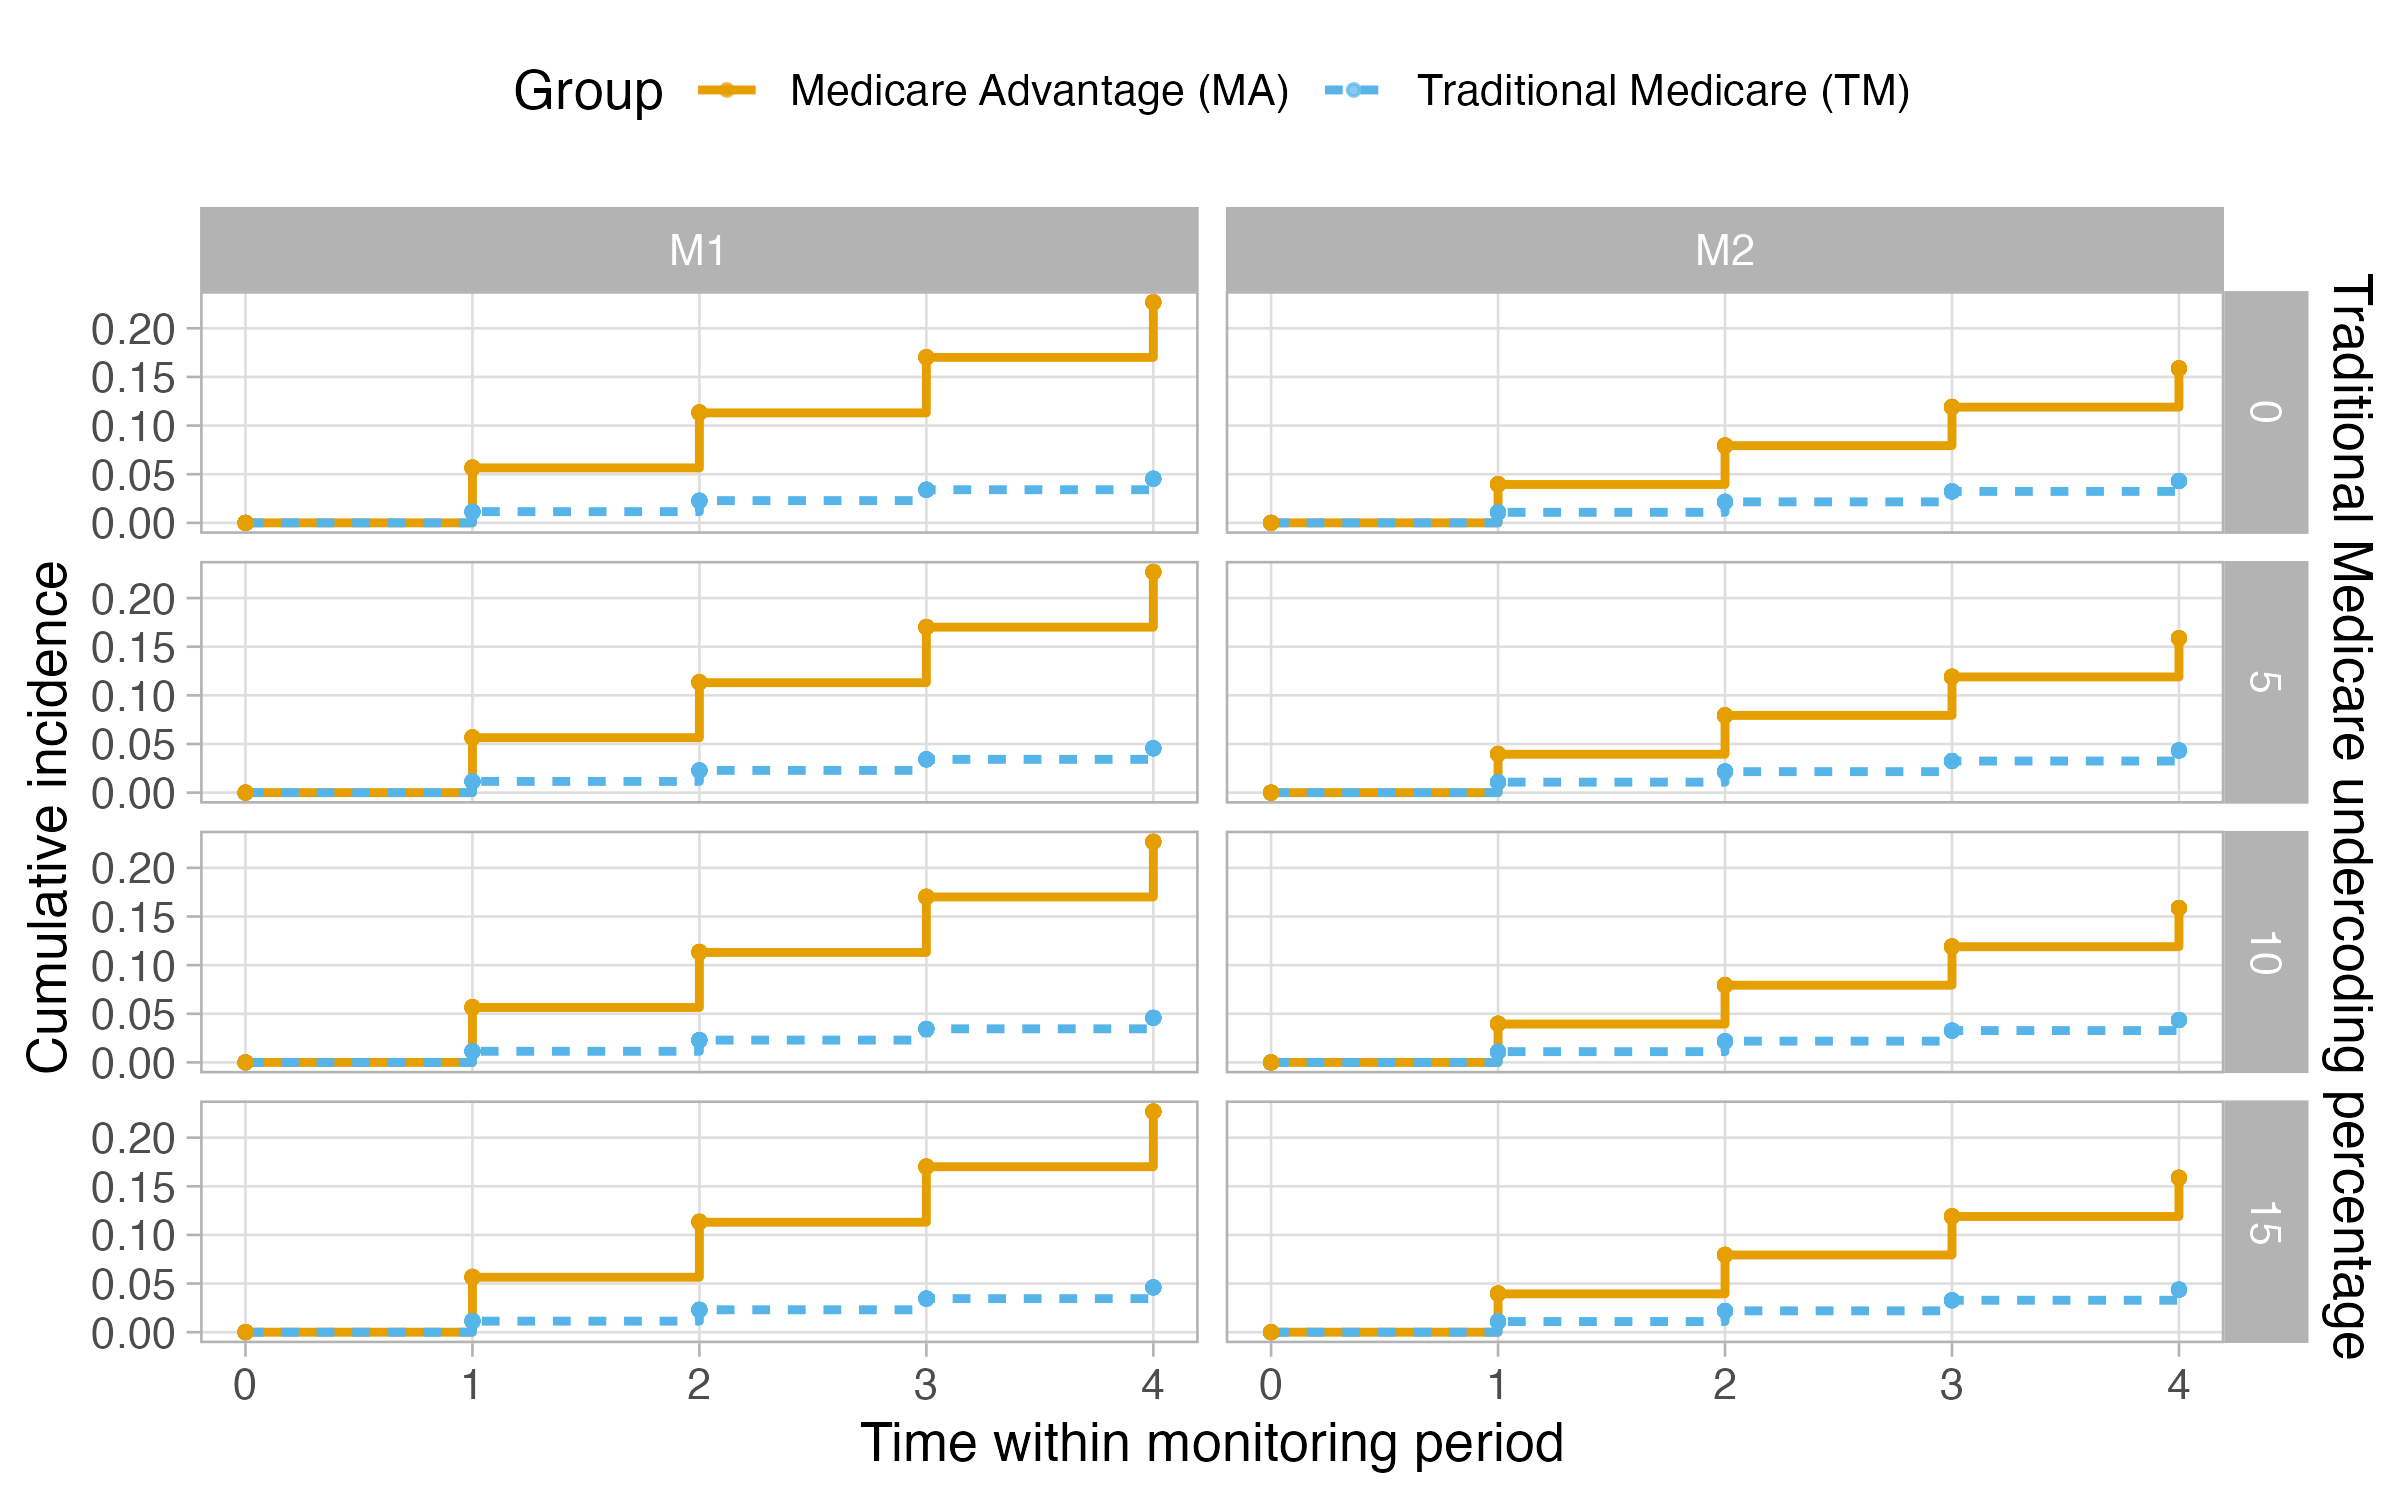
\includegraphics[keepaspectratio]{images/enache_supp_section2_figure1.png}}

}

\caption{\label{fig-supp-2-1}\textbf{Cumulative incidence functions for
the Specified Heart Arrhythmias Hierarchical Condition Category (HCC) in
simulated Medicare Advantage (MA) and Traditional Medicare (TM) groups:
25\% any-available MA upcoding.} Specified heart arrhythmias corresponds
to HCC238, which does not have any competing events. For this HCC, 25\%
of any-available individuals in the MA group are upcoded and 5\% of
any-available individuals in the TM comparison group are upcoded. The
first monitoring period is labeled M1, and the second monitoring period
is labeled M2. Given the large sample size, confidence intervals are
very narrow and are therefore omitted as they cannot be distinguished
visually.}

\end{figure}%

\begin{figure}[H]

\centering{

\pandocbounded{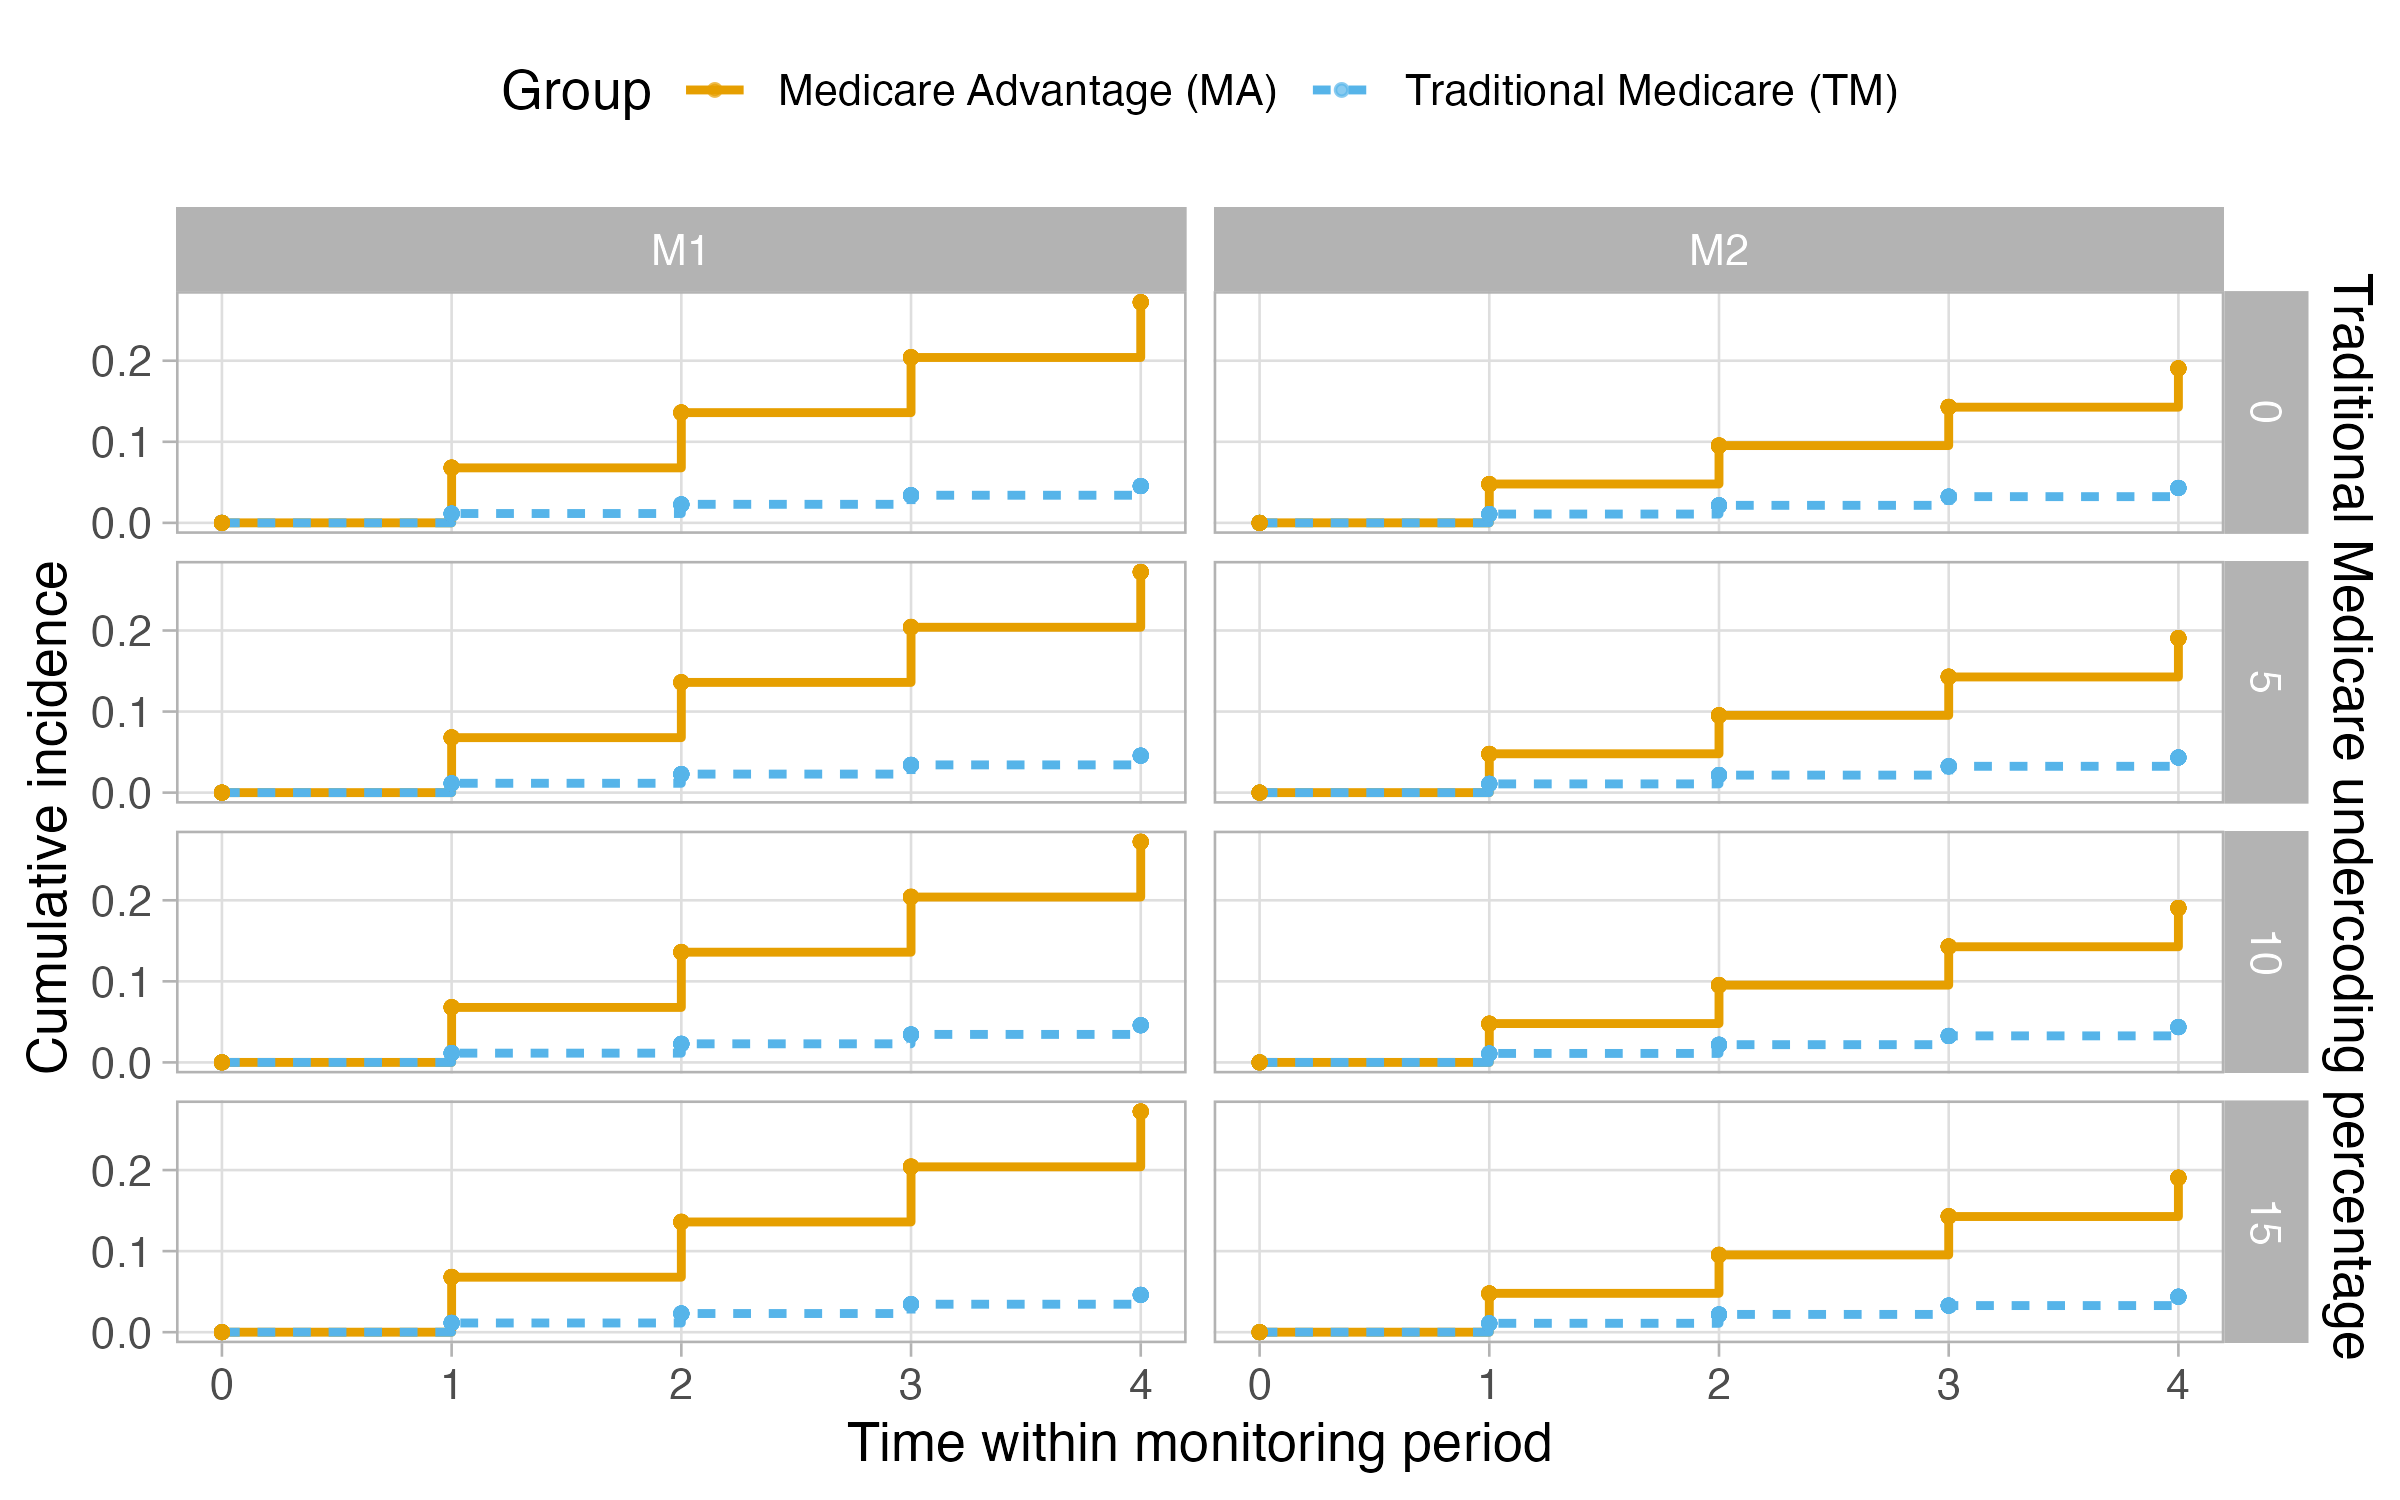
\includegraphics[keepaspectratio]{images/enache_supp_section2_figure2.png}}

}

\caption{\label{fig-supp-2-2}\textbf{Cumulative incidence functions for
the Specified Heart Arrhythmias Hierarchical Condition Category (HCC) in
simulated Medicare Advantage (MA) and Traditional Medicare (TM) groups:
30\% any-available MA upcoding.} Specified heart arrhythmias corresponds
to HCC238, which does not have any competing events. For this HCC, 30\%
of any-available individuals in the MA group are upcoded and 5\% of
any-available individuals in the TM comparison group are upcoded. The
first monitoring period is labeled M1, and the second monitoring period
is labeled M2. Given the large sample size, confidence intervals are
very narrow and are therefore omitted as they cannot be distinguished
visually.}

\end{figure}%

\begin{figure}[H]

\centering{

\pandocbounded{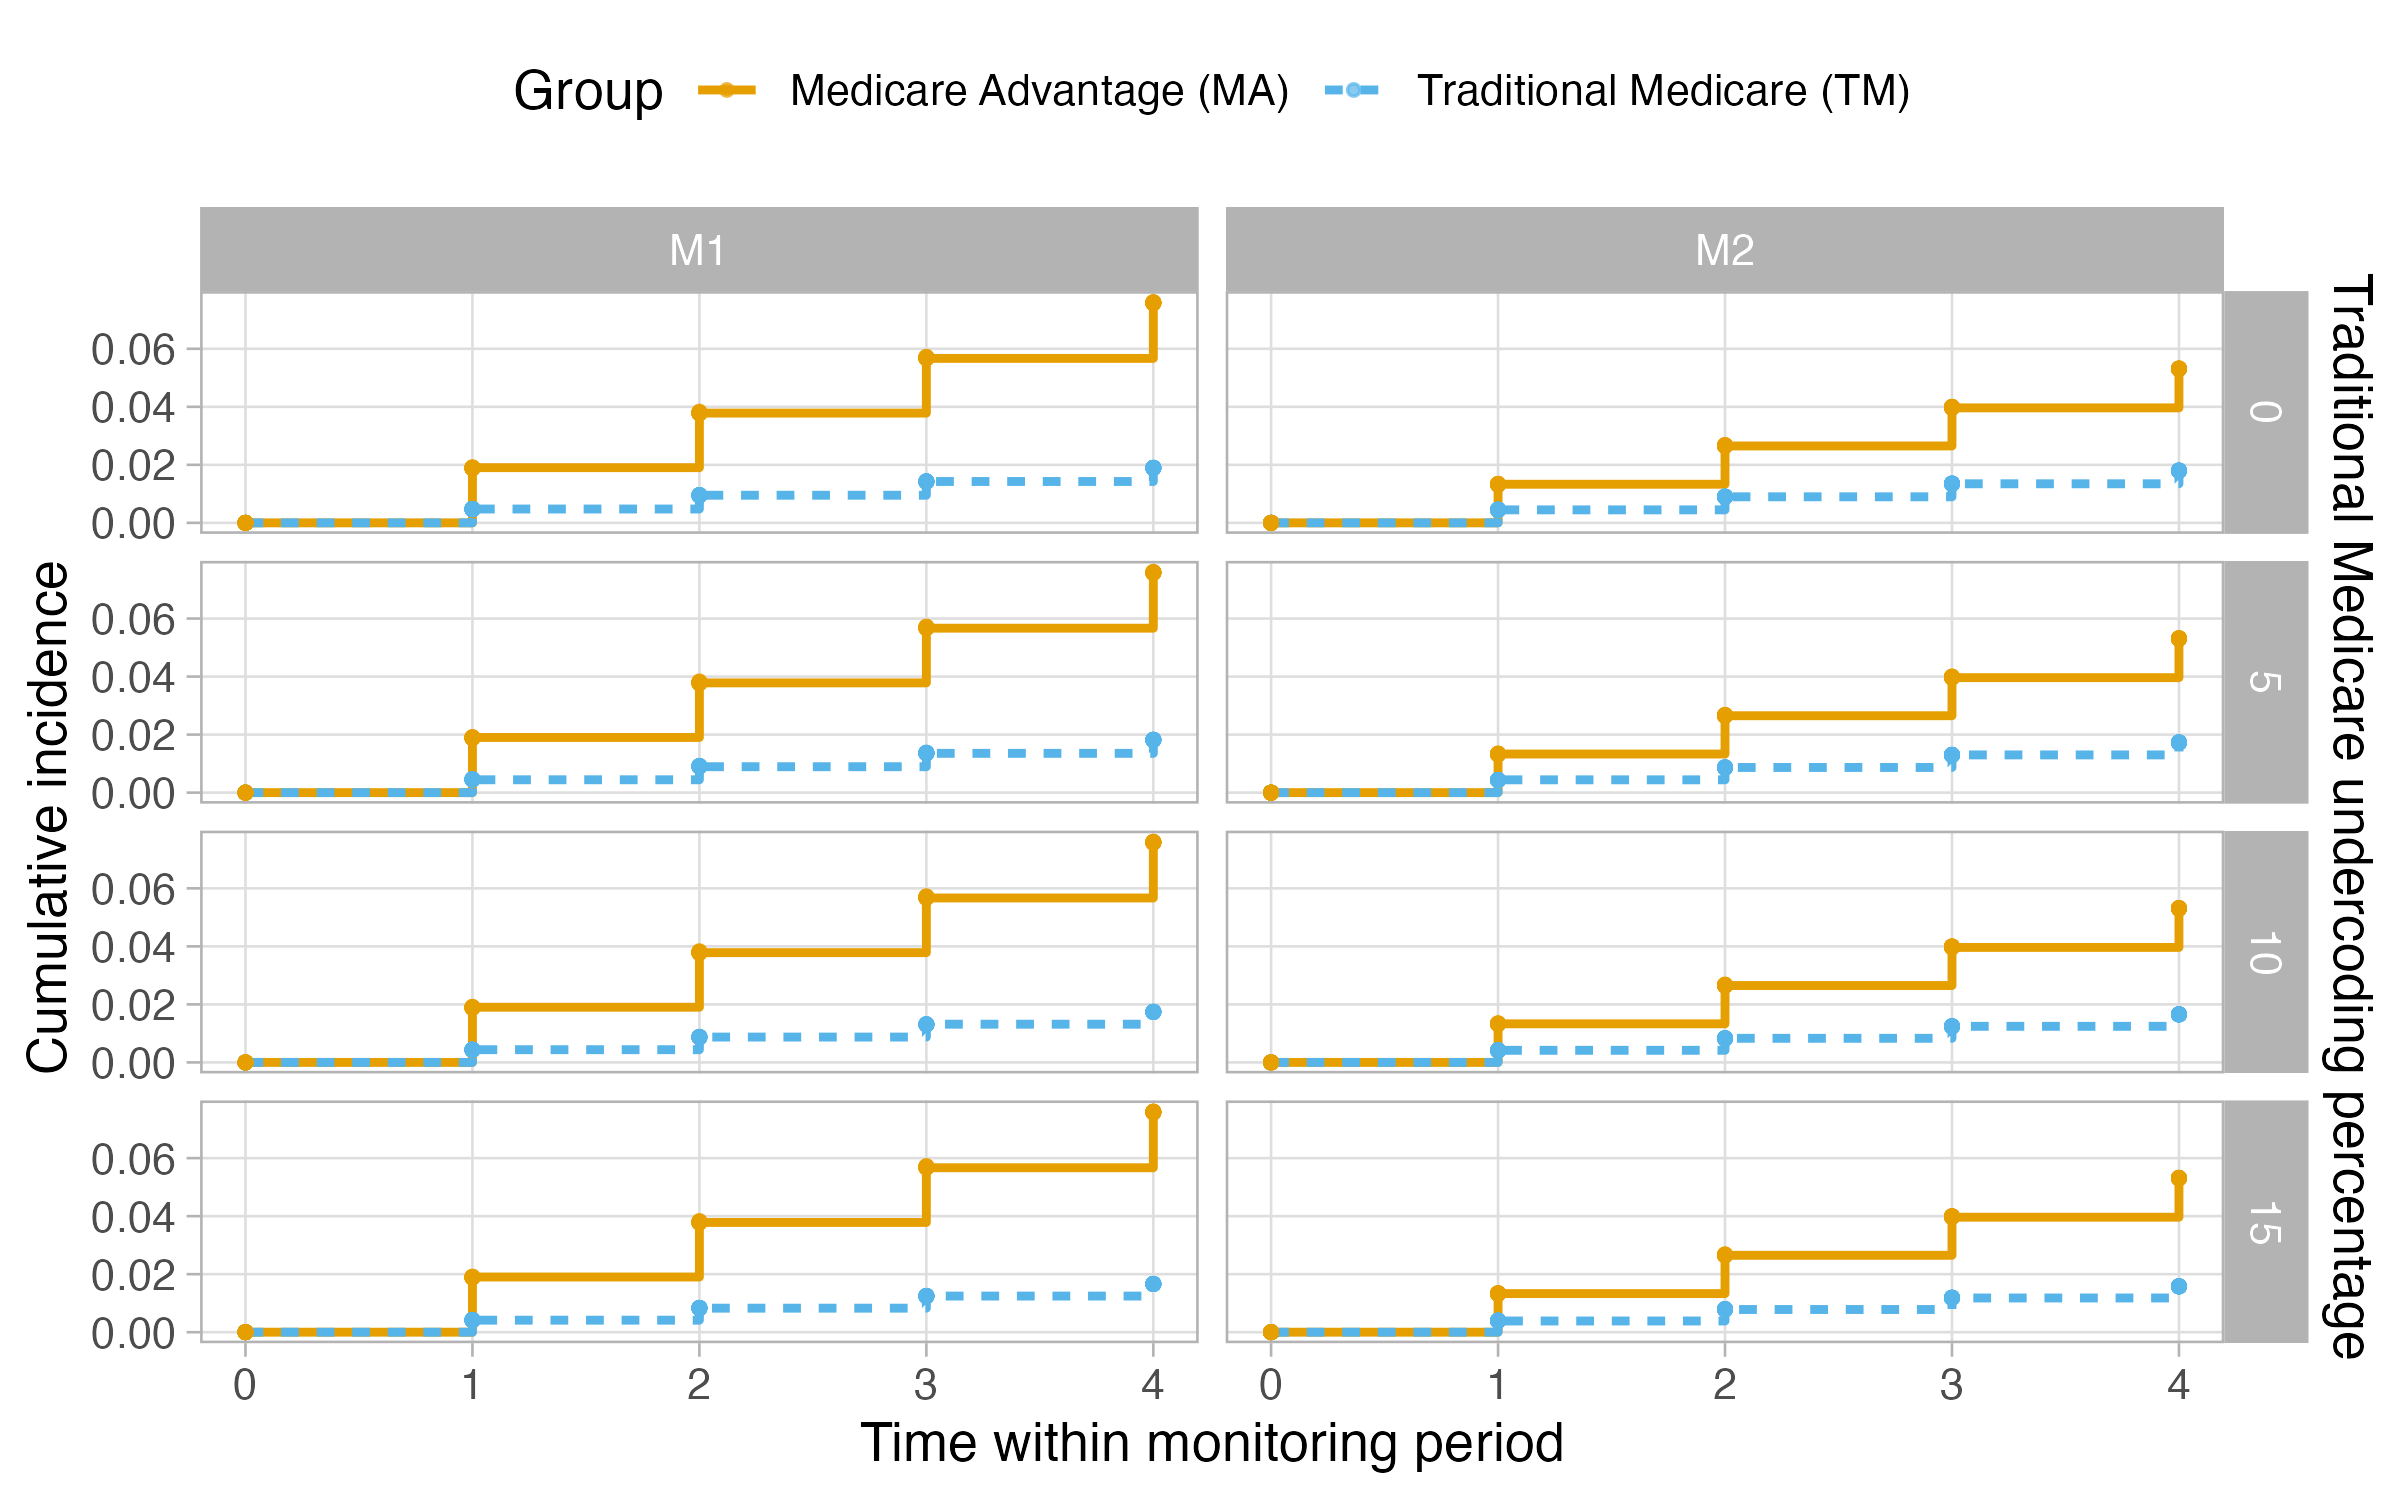
\includegraphics[keepaspectratio]{images/enache_supp_section2_figure3.png}}

}

\caption{\label{fig-supp-2-3}\textbf{Cumulative incidence functions for
the `Dementia, Severe' Hierarchical Condition Category (HCC) in
simulated Medicare Advantage (MA) and Traditional Medicare (TM) groups:
20\% lower severity MA upcoding.} `Dementia, Severe' corresponds to
HCC125, which has lower severity HCCs `Dementia, Moderate' (HCC126) and
`Dementia, Mild or Unspecified' (HCC127). 20\% of any individuals in the
MA group who were previously coded with either HCC126 or HCC127 are
upcoded and 5\% of individuals in the TM comparison group are upcoded
similarly. The first monitoring period is labeled M1, and the second
monitoring period is labeled M2. Given the large sample size, confidence
intervals are very narrow and are therefore omitted as they cannot be
distinguished visually.}

\end{figure}%

\begin{figure}[H]

\centering{

\pandocbounded{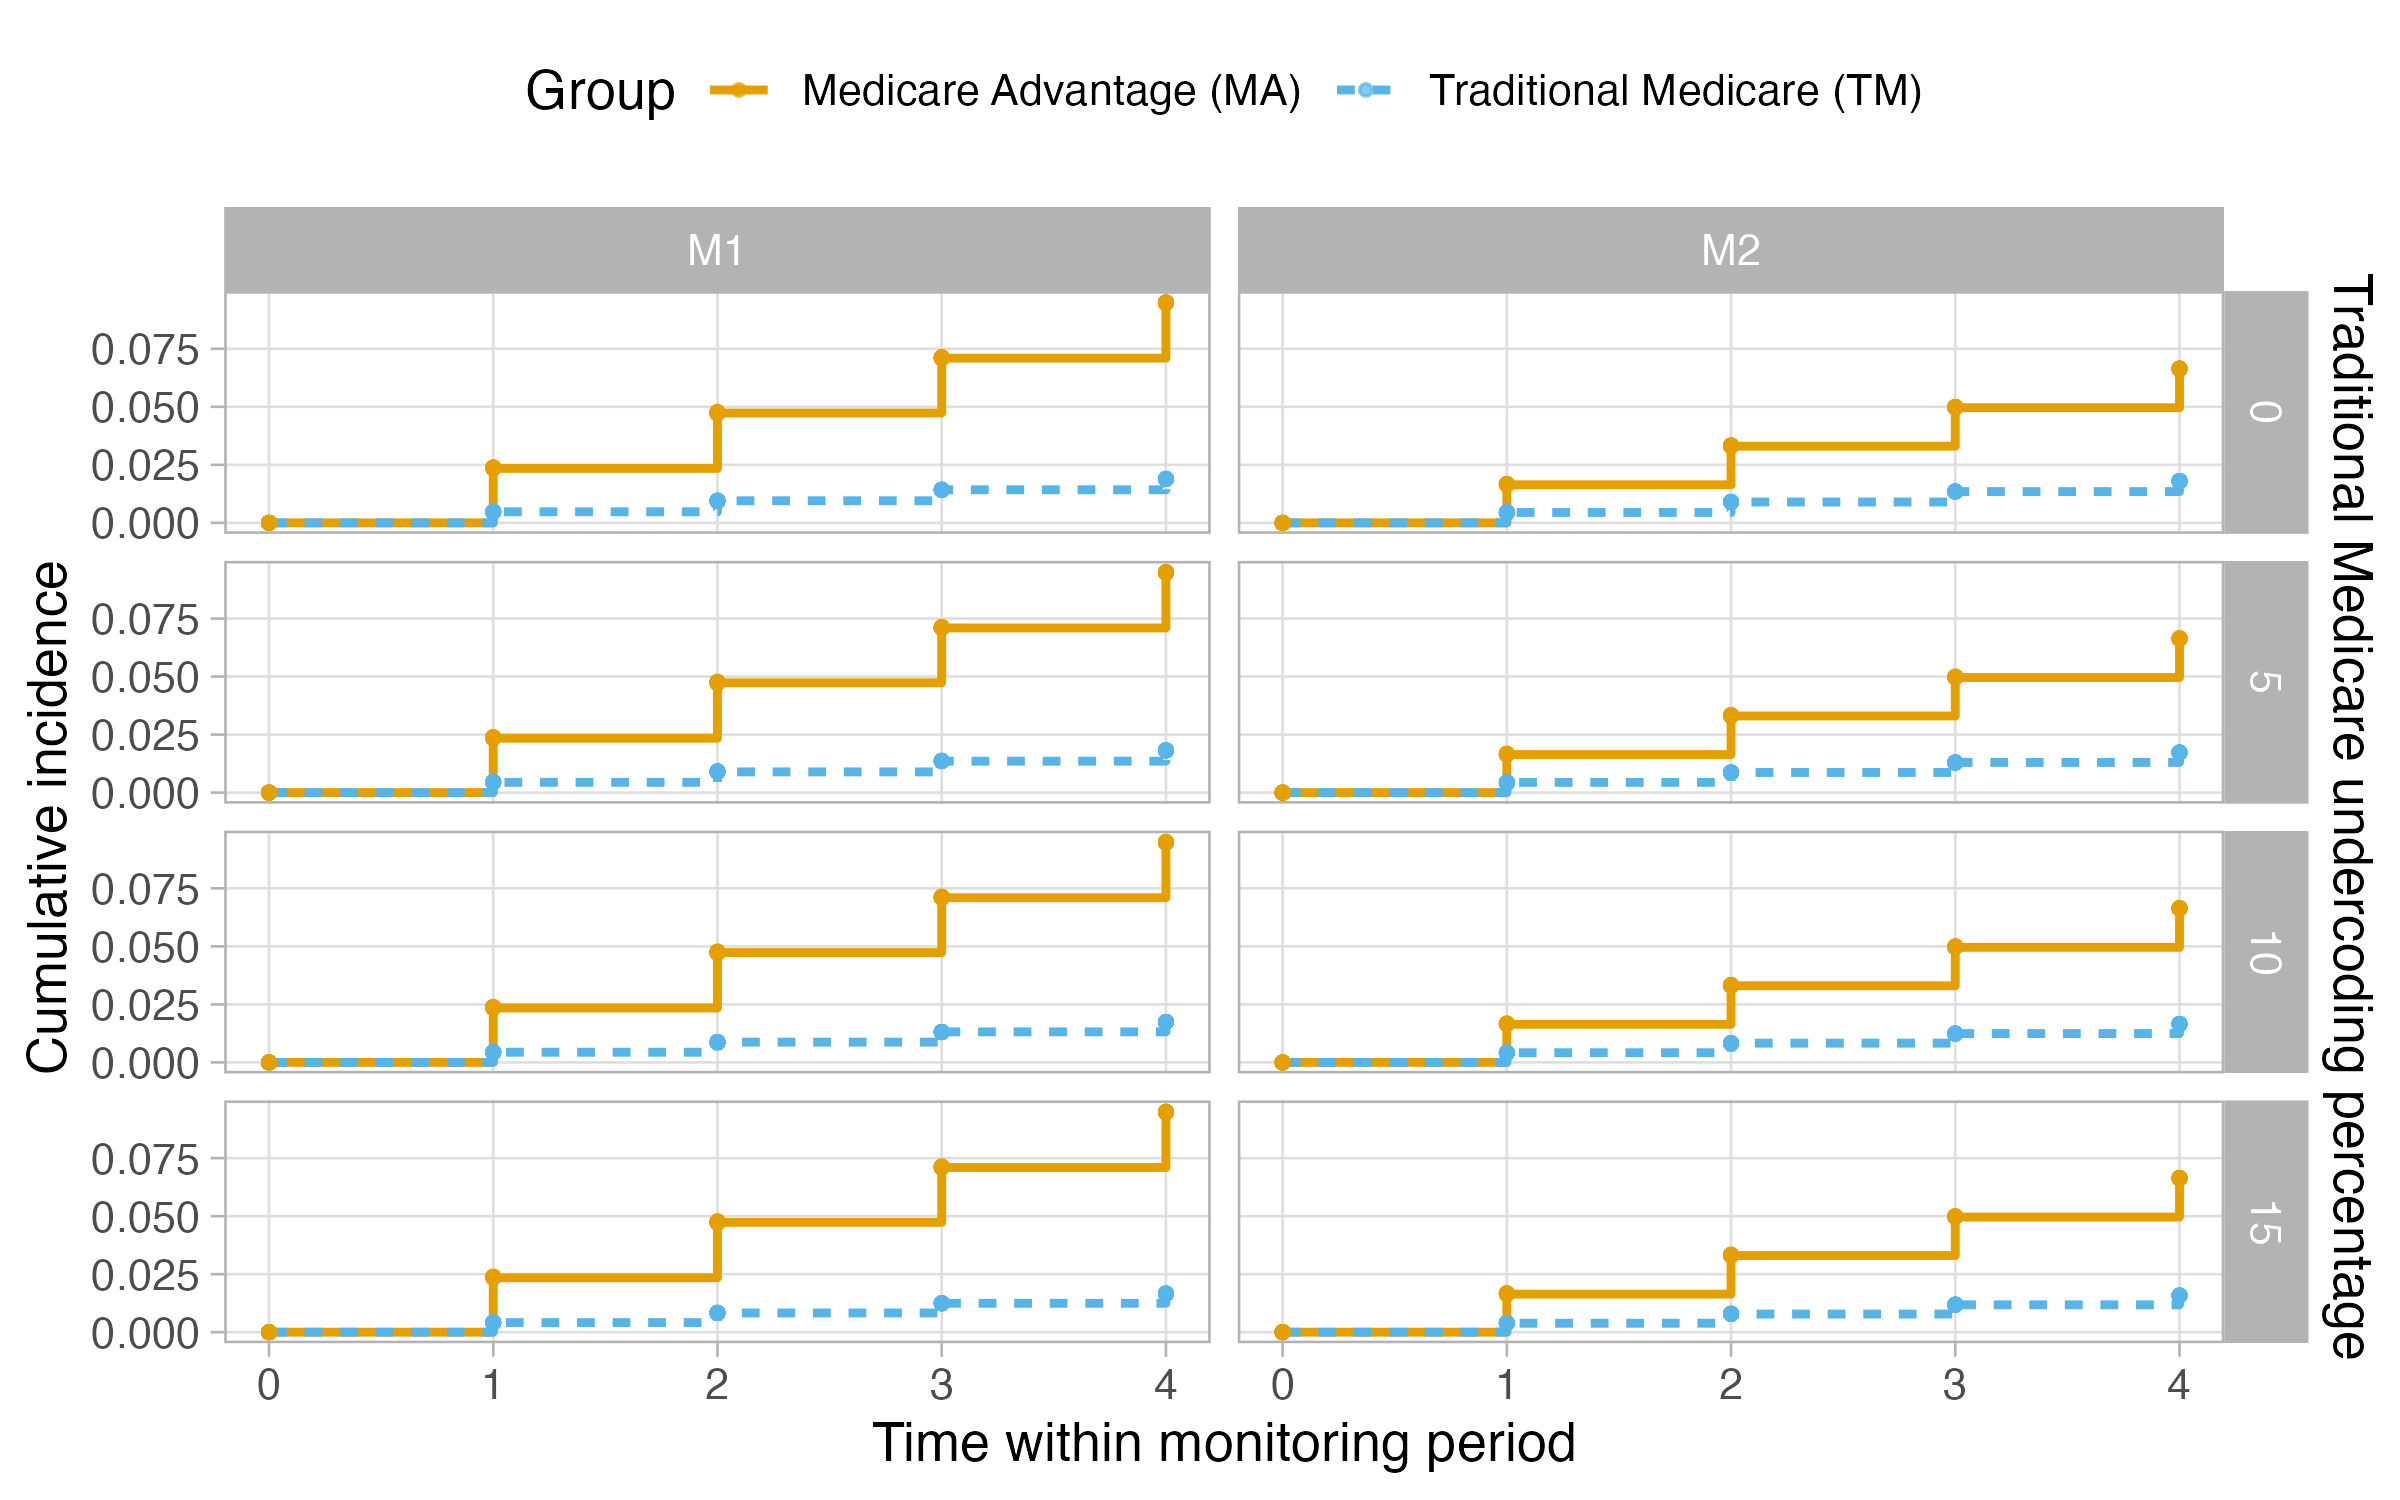
\includegraphics[keepaspectratio]{images/enache_supp_section2_figure4.png}}

}

\caption{\label{fig-supp-2-4}\textbf{Cumulative incidence functions for
the `Dementia, Severe' Hierarchical Condition Category (HCC) in
simulated Medicare Advantage (MA) and Traditional Medicare (TM) groups:
25\% lower severity MA upcoding.} `Dementia, Severe' corresponds to
HCC125, which has lower severity HCCs `Dementia, Moderate' (HCC126) and
`Dementia, Mild or Unspecified' (HCC127). 25\% of any individuals in the
MA group who were previously coded with either HCC126 or HCC127 are
upcoded and 5\% of individuals in the TM comparison group are upcoded
similarly. The first monitoring period is labeled M1, and the second
monitoring period is labeled M2. Given the large sample size, confidence
intervals are very narrow and are therefore omitted as they cannot be
distinguished visually.}

\end{figure}%

\begin{figure}[H]

\centering{

\pandocbounded{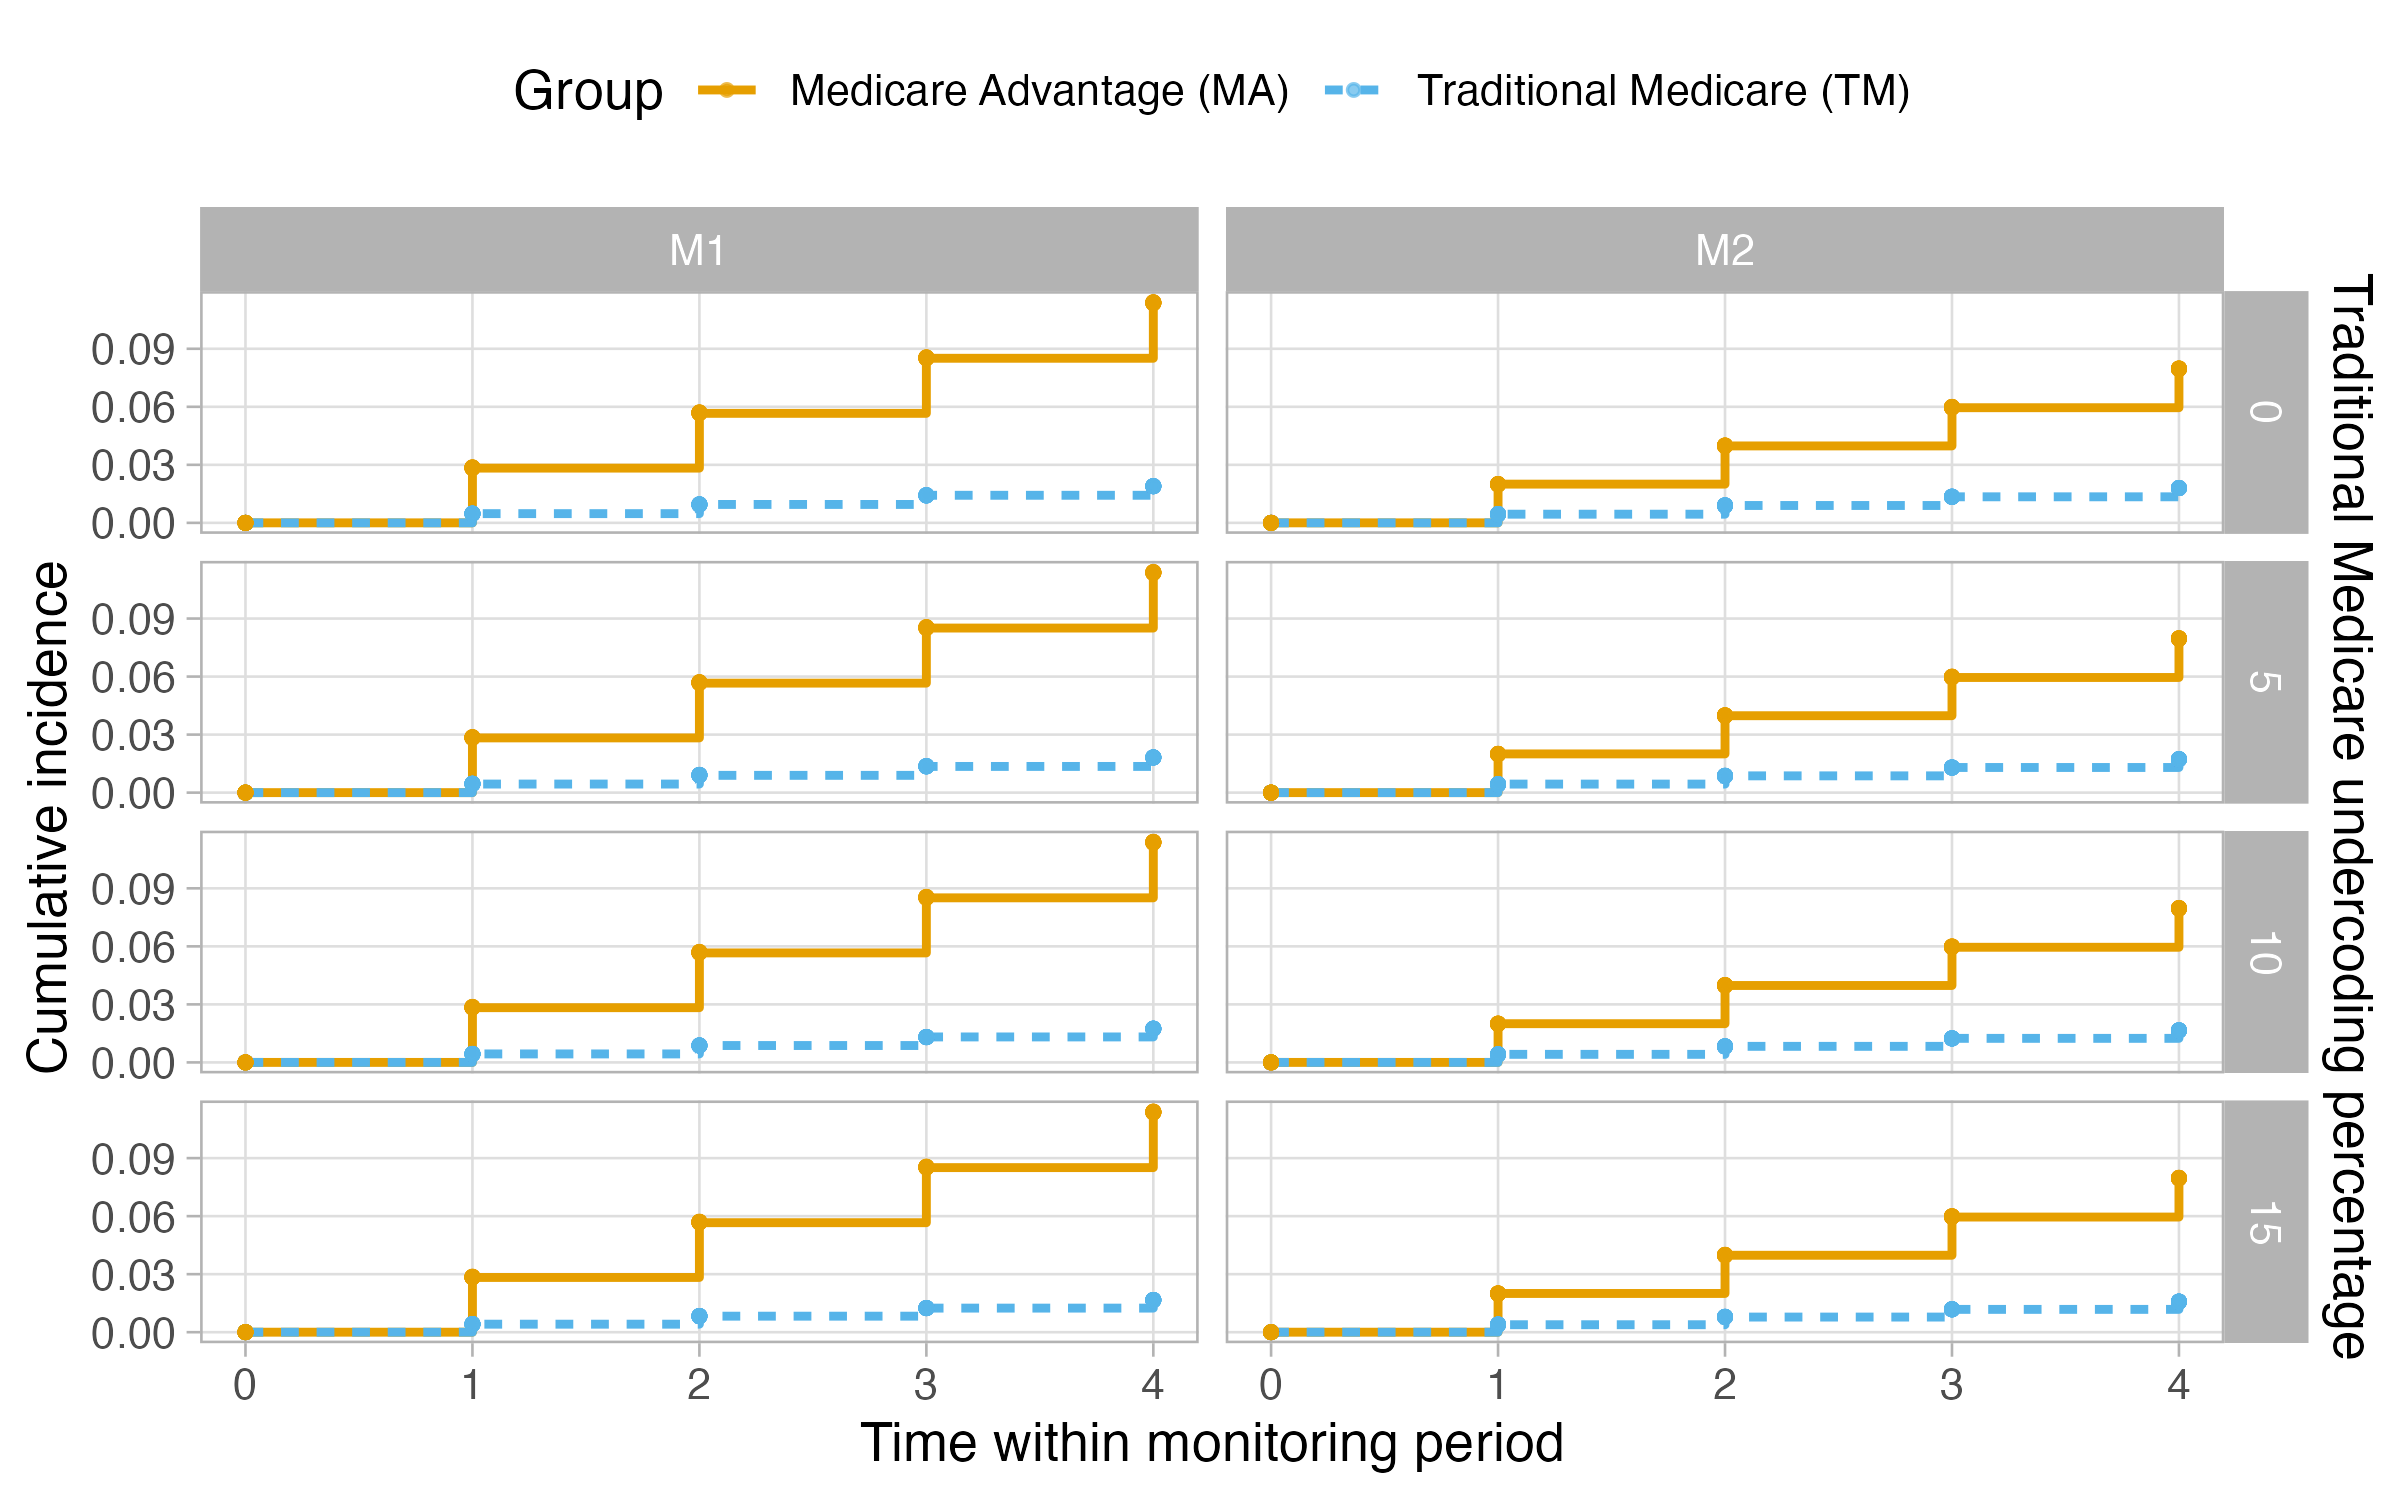
\includegraphics[keepaspectratio]{images/enache_supp_section2_figure5.png}}

}

\caption{\label{fig-supp-2-5}\textbf{Cumulative incidence functions for
the `Dementia, Severe' Hierarchical Condition Category (HCC) in
simulated Medicare Advantage (MA) and Traditional Medicare (TM) groups:
30\% lower severity MA upcoding.} `Dementia, Severe' corresponds to
HCC125, which has lower severity HCCs `Dementia, Moderate' (HCC126) and
`Dementia, Mild or Unspecified' (HCC127). 30\% of any individuals in the
MA group who were previously coded with either HCC126 or HCC127 are
upcoded and 5\% of individuals in the TM comparison group are upcoded
similarly.The first monitoring period is labeled M1, and the second
monitoring period is labeled M2. Given the large sample size, confidence
intervals are very narrow and are therefore omitted as they cannot be
distinguished visually.}

\end{figure}%

\begin{figure}[H]

\centering{

\pandocbounded{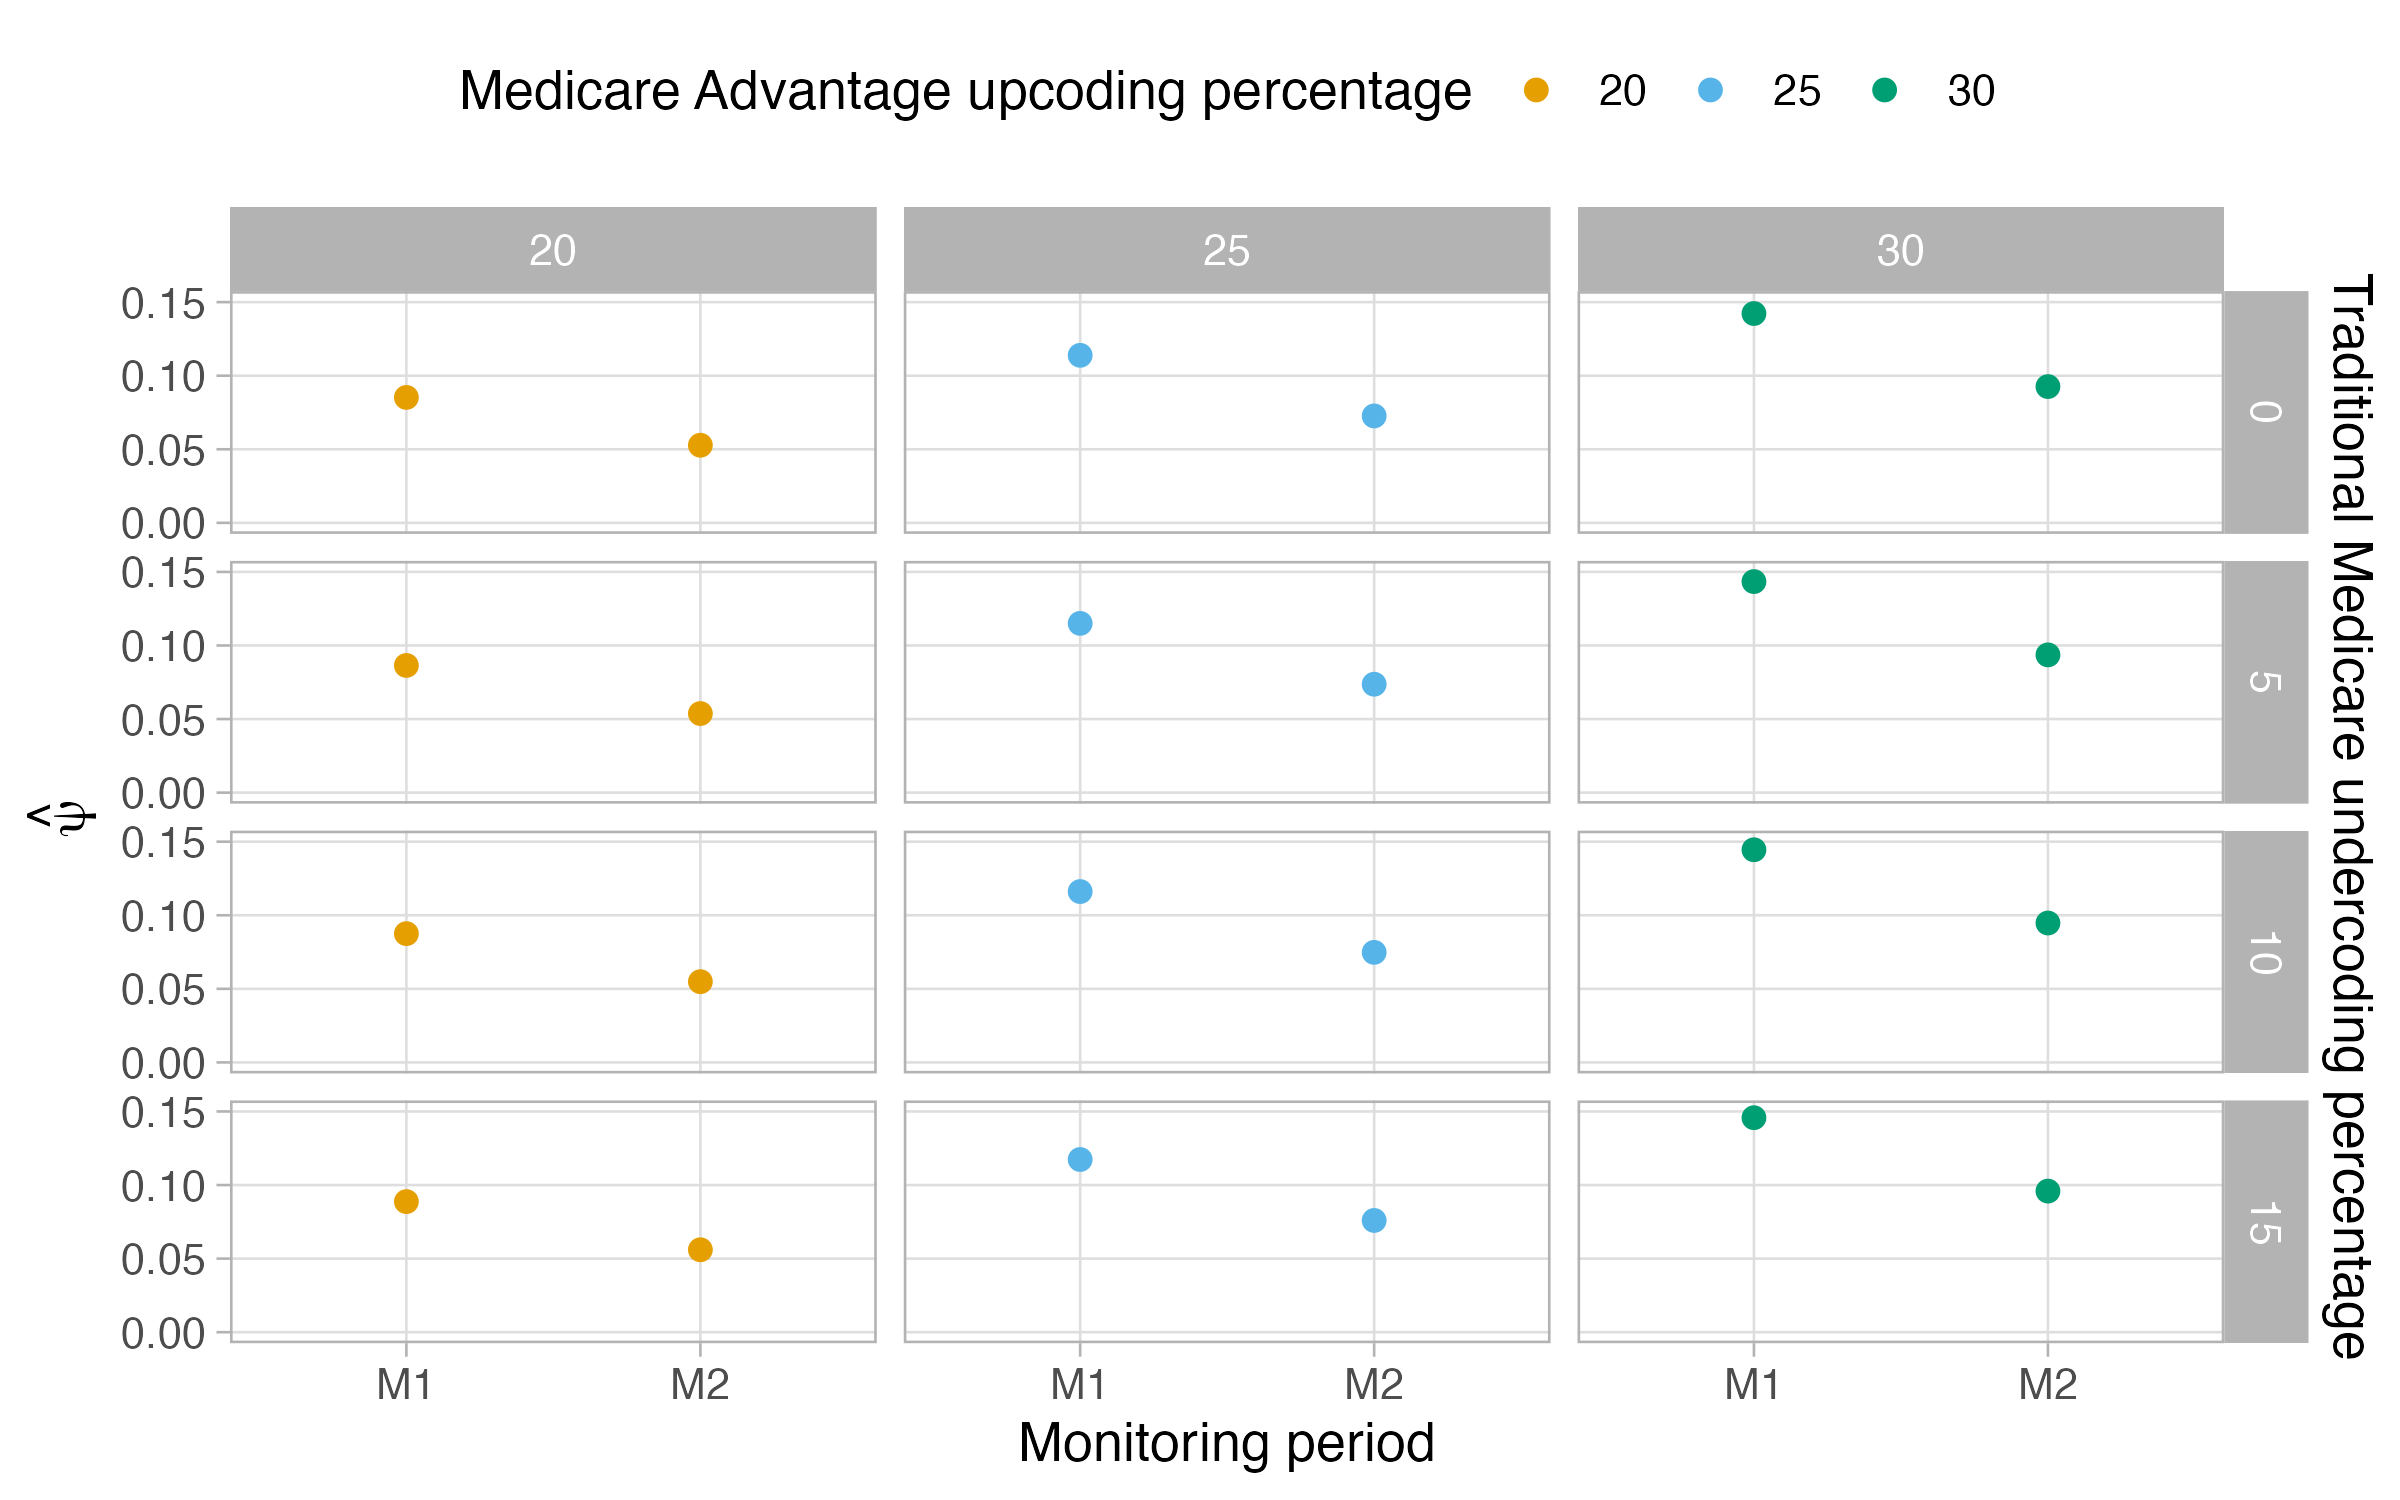
\includegraphics[keepaspectratio]{images/enache_supp_section2_figure6.png}}

}

\caption{\label{fig-supp-2-6}\textbf{Within-monitoring period}
\(\boldsymbol{\psi}\) \textbf{estimates for the `Dementia, Severe'
Hierarchical Condition Category (HCC) in simulated Medicare Advantage
(MA) and Traditional Medicare (TM) groups.} \(\widehat{\psi}\)
corresponds to the proposed estimator for \(\psi\), or the difference in
mean time without event (i.e.~incident coding of the HCC) across groups.
`Dementia, Severe' corresponds to HCC125, which has lower severity HCCs
`Dementia, Moderate' (HCC126) and `Dementia, Mild or Unspecified'
(HCC127). For this HCC, individuals in the MA group who were previously
coded with either HCC126 or HCC127 are upcoded to varying degrees and
individuals in the TM comparison group are upcoded 5\% similarly. The
first monitoring period is labeled M1, and the second monitoring period
is labeled M2. Given the large sample size, confidence intervals are
very narrow and are therefore omitted as they cannot be distinguished
visually.}

\end{figure}%

\newpage{}

\textbf{References}

\phantomsection\label{refs}
\begin{CSLReferences}{0}{1}
\bibitem[\citeproctext]{ref-Ellis2018-mr}
\CSLLeftMargin{1. }%
\CSLRightInline{Ellis RP, Martins B, Rose S. {Chapter 3 - Risk
Adjustment for Health Plan Payment}. In: McGuire TG, Kleef RC van, eds.
\emph{{Risk Adjustment, Risk Sharing and Premium Regulation in Health
Insurance Markets}}. Academic Press; 2018:55-104.
doi:\href{https://doi.org/10.1016/B978-0-12-811325-7.00003-8}{10.1016/B978-0-12-811325-7.00003-8}}

\bibitem[\citeproctext]{ref-Ghoshal-Datta2024-io}
\CSLLeftMargin{2. }%
\CSLRightInline{Ghoshal-Datta N, Chernew ME, McWilliams JM. {Lack of
Persistent Coding in Traditional Medicare May Widen the Risk-Score Gap
with Medicare Advantage}. \emph{Health Aff}. 2024;43(12):1638-1646.
doi:\href{https://doi.org/10.1377/hlthaff.2024.00169}{10.1377/hlthaff.2024.00169}}

\bibitem[\citeproctext]{ref-Conner2021-ac}
\CSLLeftMargin{3. }%
\CSLRightInline{Conner SC, Trinquart L. {Estimation and Modeling of the
Restricted Mean Time Lost in the Presence of Competing Risks}.
\emph{Stat Med}. 2021;40(9):2177-2196.
doi:\href{https://doi.org/10.1002/sim.8896}{10.1002/sim.8896}}

\bibitem[\citeproctext]{ref-theall2019}
\CSLLeftMargin{4. }%
\CSLRightInline{All of Us Research Program Investigators. {The {``All of
Us''} Research Program}. \emph{N Engl J Med}. 2019;381(7):668-676.
doi:\href{https://doi.org/10.1056/NEJMsr1809937}{10.1056/NEJMsr1809937}}

\bibitem[\citeproctext]{ref-Barberio2024-vs}
\CSLLeftMargin{5. }%
\CSLRightInline{Barberio J, Naimi AI, Patzer RE, et al. {Influence of
Incomplete Death Information on Cumulative Risk Estimates in US Claims
Data}. \emph{Am J Epidemiol}. 2024;193(9):1281-1290.
doi:\href{https://doi.org/10.1093/aje/kwae034}{10.1093/aje/kwae034}}

\bibitem[\citeproctext]{ref-Centers_for_Medicare_and_Medicaid_Services2023-zf}
\CSLLeftMargin{6. }%
\CSLRightInline{Centers for Medicare \& Medicaid Services. {Advance
Notice of Methodological Changes for Calendar Year (CY) 2024 for
Medicare Advantage (MA) Capitation Rates and Part C and Part D Payment
Policies}. Published online February 1, 2023. Accessed June 15, 2024.
\url{https://www.cms.gov/files/document/2024-advance-notice-pdf.pdf}}

\bibitem[\citeproctext]{ref-Centers-for-Medicare-and-Medicaid-ServicesUnknown-pf}
\CSLLeftMargin{7. }%
\CSLRightInline{Centers for Medicare and Medicaid Services. 2024 model
software/{ICD}-10 mappings, 2024 midyear/final model software. Published
online 2024. Accessed December 4, 2024.
\url{https://www.cms.gov/medicare/health-plans/medicareadvtgspecratestats/risk-adjustors/2024-model-software/icd-10-mappings}}

\end{CSLReferences}




\end{document}
